\documentclass[ms,thesis,twoside]{iist}

%% ---- Packages of use ---- %%

\usepackage[pdftex]{graphicx}
\usepackage[backend=biber, citestyle=authoryear, style=authoryear]{biblatex}
\usepackage{booktabs}
\usepackage{colortbl}
\usepackage{csquotes}
\usepackage{float}
\usepackage{layouts}
\usepackage{pdflscape}
\usepackage{subcaption}
\usepackage[normalem]{ulem}

%% ---- Figure Management ---- %%

\graphicspath{{./figures/}}

%% ---- Bibliography Management ---- %%

\addbibresource{doct.bib}

\title{Multimessenger constraints on outflows from neutron star mergers}
\author{B.S.Bharath Saiguhan}
\studentid{SC16B123}
\advisor{Dr. Resmi Lekshmi}
\specialization{Astronomy and Astrophysics}
\department{Earth and Space Sciences}
\date{\today}


%% ---- Document starts here ---- %%
\begin{document}

    \raggedbottom

    %% ---- Make the initial set of pages ---- %%

    \maketitle % Title page
    \makecertificate % Certificate
    \makedeclaration % Declaration
    \makededication % Dedication -- DONE
    \makeacknowledgements % Acknowledgements -- TODO
    \makeabstract % Abstract -- TODO
    \maketableofcontents % Table of contents -- TODO
    \makelistoffigures % List of figures -- TODO
    \makelistoftables % List of tables -- TODO
    %\makelistofalgorithms % List of algorithms -- TODO
    \makeabbreviations % List of abbreviations -- TODO
    %\makenomenclature % Nomenclature (for symbols used) -- TODO

    % Initialize chapter settings; DO NOT comment this line

    \makechaptersettings

    %% ---- Start chapters here ---- %%

    \chapter{Introduction}\label{ch:introduction}

\section{Outflows from BNS Mergers}\label{sec:bns}
    Due to the joint electromagnetic and gravitational wave detection of the binary
    neutron star merger event GW1701817 (see \cite{abbott_2018}), there has
    been renewed interest in SGRBs.  Specifically, this detection gives credence to the
    claim that the central engines of SGRBs are binary neutron star mergers (see
    \cite{narayan_1992}). However, there are other aspects of the process that
    are not as clear. Specifically, several aspects of GW170817 have not been completely
    explained. The main concerns are as follows (\cite{lazzati_2020}):

    \begin{itemize}

        \item The outflow of GRB170817A was lower in energy than a typical cosmological
            SGRB, by a factor of $10^4 - 10^5$, even though the event was one of the
            closest GW events recorded, at a distance of $\sim$ 40 Mpc. This could be
            due to two factors :

            \begin{itemize}

                \item The structured jet was off-axis with respect to the observer.

                \item The internal engine powering this SGRB was intrinsically less
                    energetic, and differs from the one observed in other typical SGRBs.

            \end{itemize}

        \item A clear consensus has not been reached on how the gamma-ray prompt
            emission was produced. The uncertainty partly comes from the fact that the
            various delays involved before the prompt emission is observed are not
            accurately constrained. Models which have been considered include :

            \begin{itemize}

                \item The structured outflow model, characterised by functions for the
                    Lorentz factor and the energy per unit solid angle, both of which
                    vary with the angle made with the polar jet axis ($\theta$). This
                    model produces detectable signals even at moderately large off-axis
                    angles.

                \item The shock breakout model, wherein the leading edge of the wind
                    emits the prompt emission as it breaks out of the cocoon of nuclear
                    matter ejected before the jet was launched. This model has been
                    shown to explain the energetics and spectrum of the prompt emission,
                    although it does require a setup in which the wind is fast enough so
                    that it can reach a large enough distance at breakout.

            \end{itemize}

    \end{itemize}

    More light can be shed on these questions by observing more such SGRBs, using both
    the gravitational wave (GW) and electromagnetic (EM) windows.  However, the
    possibility of joint detections are slim, due to the fact that the EM observations
    are highly dependent on the viewing angle of the system with respect to the observer
    (due to relativistic beaming), whereas GW signal amplitudes depend on the distance
    to the event (see ).\\
    Given that this is the case, it would be expedient to look for constraints on the
    structure parameters of various models.  Furthermore, it would be useful to develop
    models which are resilient to non-detections, and can produce constraints on the
    parameters using even upper limits on the flux/fluence observed by the various EM
    follow-up satellites, such as INTEGRAL, Fermi or Swift.\\

    \subsection{Modelling outflows from BNS Mergers}\label{ssec:bns-outflows}

    As mentioned before, the electromagnetic follow-up of the binary neutron star merger
    event GW170817 helped measure the various time delays between the time of the GW
    signal trigger (which roughly is the merger time itself) and the time the gamma-ray
    signals were picked up. This time delay is denoted $\Delta t_{GW-\gamma}$, and was
    around 1.75 seconds for this event.  The components which make up this delay are as
    follows (\cite{lazzati_2020}):

    \begin{itemize}

        \item \textbf{Engine Delay} -- this is the delay due to a transition mechanism
            in the central engine which powers the jet (such as a metastable, fast
            spinning neutron star collapsing into a black hole when its rotation period
            increases; this process can take years) or due to the time elapsed in
            amplifying the magnetic field to a value large enough for jet launching
            (this process is significantly faster, taking only seconds). This is denoted
            by $\Delta t_{eng}$.

        \item \textbf{Wind Delay} -- this is simply a delay in the launching of a
            non-relativistic wind due to the neutron-rich matter from the progenitor(s)
            being tidally shredded. For this reason, it can be \textit{negative} as
            well, since the tidal shredding can occur before the merger itself. This is
            denoted as $\Delta t_{wind}$.

        \item \textbf{Breakout Delay} -- if the wind is ejected before the jet, then the
            latter will have to propagate through the former. This happens at a
            sub-relativistic speed, whereas the GW signal travels at a relativistic
            speed. The delay due to this crossing is the breakout delay, and is denoted
            $\Delta t_{bo}$. During this time, jet-wind interactions cause the
            development of a structured outflow that maintains a bright core but also
            has energetic wings at large polar angles.

        \item \textbf{Photospheric Delay} --  once the jet has crossed the wind, it
            still needs to propagate out to the photospheric radius, where the outflow
            becomes transparent and the prompt gamma-ray emission is radiated. The delay
            from the breakout radius to the photospheric radius is $\Delta t_{ph}$. This
            is given by (for GW170817):

            \begin{equation}
                \label{eq:4}
                \Delta t_{ph} \sim \dfrac{R_{ph}}{c \Gamma^2} =
                    1.4 \dfrac{R_{ph}}{2 \times 10^{12} \text{ cm}}
                    \left( \dfrac{7} {\Gamma} \right)^2 \text{ s}
            \end{equation}

        \item \textbf{Dissipation Delay} -- this is a requirement in some models, such
            as the internal shock synchrotron model, wherein the outflow needs to travel
            to the internal shock radius before the bulk energy of the flow is
            dissipated and turned into radiation. The time required to get to this point
            after crossing the photospheric radius is the dissipation delay, denoted
            $\Delta t_{\gamma}$

    \end{itemize}

    Several attempts to constrain the various time delay components have been made.
    However, except for relative comparisons, no conclusions have been arrived upon.
    For example, one can only say that the photospheric delay is the major component out
    of all the delays, and that wind delay (if non-zero) has to be lesser than the jet
    delay, so that the jet catches up to the wind and the jet-wind interaction generates
    the structured outflow. Fig. \ref{fig:jet_delay} summarises these delays in the
    broader context.

    \begin{figure}[H]
        \centering
        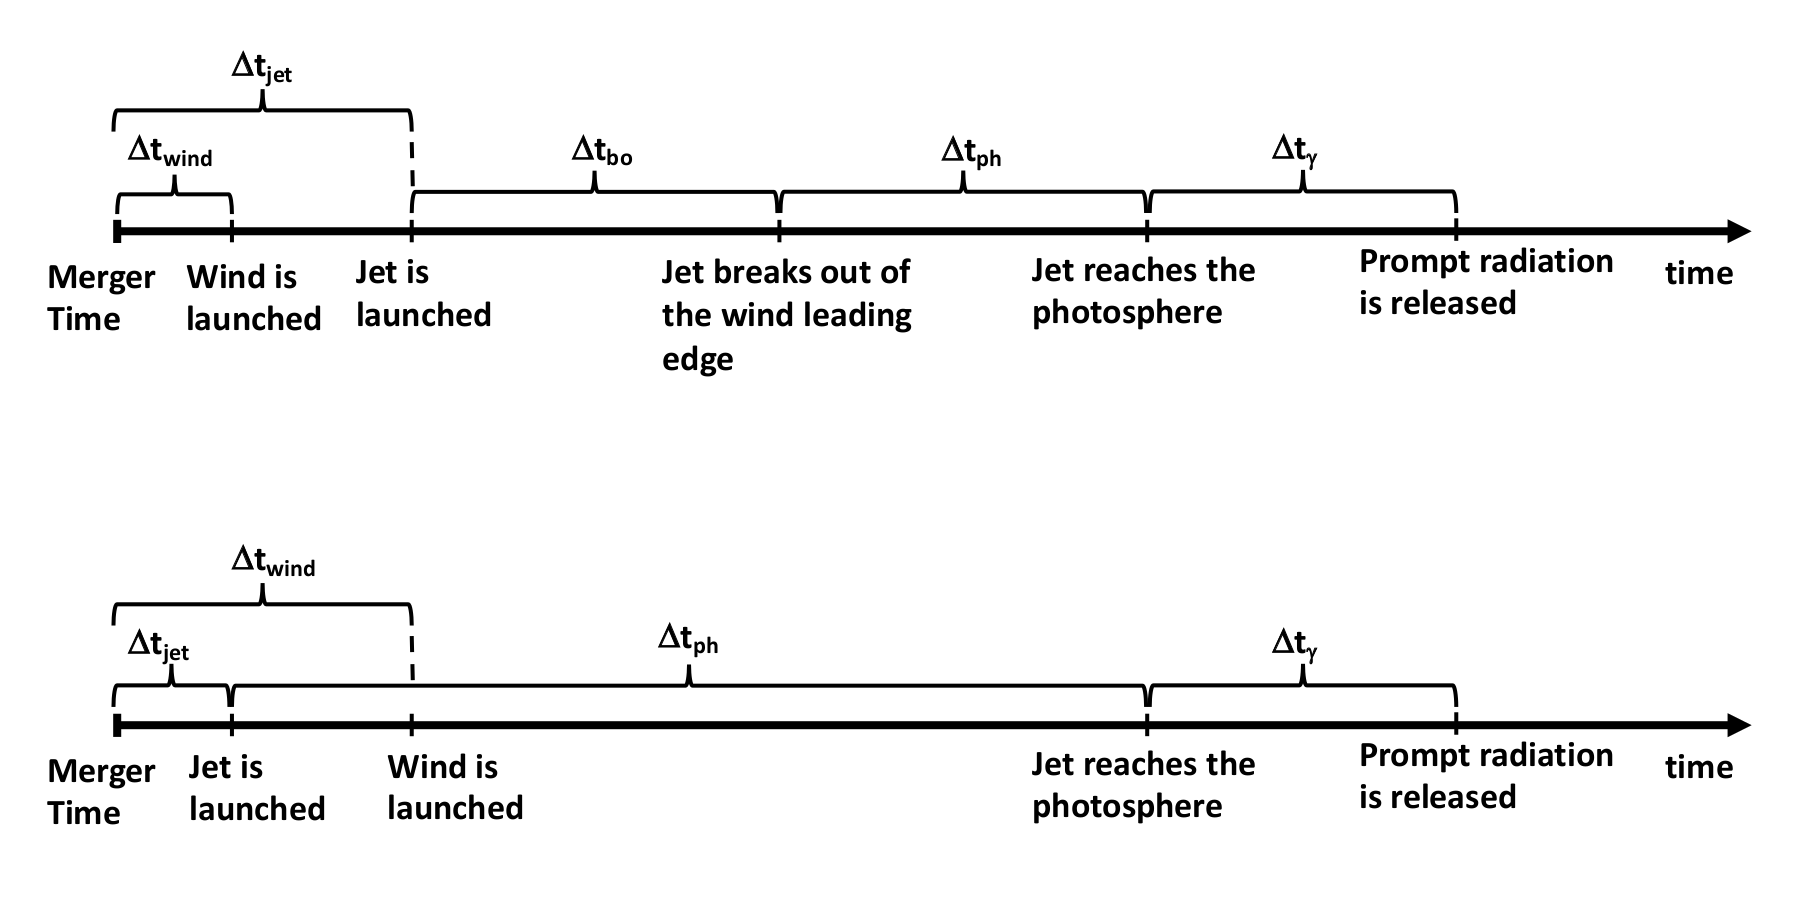
\includegraphics[width=12cm]{jet_delay}
        \caption[Relative Positions of Jet Delays]
             {
                    Two possible scenarios for the relative positioning of the delays in
                    time, which contribute to $\Delta t_{GW-\gamma}$.  Owing to the
                    requirement of a structured outflow, GW170817 possibly follows the
                    top timeline. The relative contributions of the various delays are
                    debated, but it is agreed that $\Delta t_{wind} < \Delta t_{jet} \ll
                    1$ s, $\Delta t_{bo} \ll 1$ s, $\Delta t_{\gamma} \sim 0$ and
                    $\Delta t_{ph} \sim \Delta t_{GW-\gamma}$.
             }
        \label{fig:jet_delay}
    \end{figure}

    Due to the uncertainties in the delay terms, several models for the jet can explain
    the energetics and observed structure. Numerical simulations are also unequivocal
    about their favouring of one model over the other (see \cite{shibata_2019}).
    Some models try to explain the \textit{apparent} structure of the jet, which are the
    observables seen by a particular observer at a particular viewing angle. Other
    models are used to explain the \textit{intrinsic} structure, such as the polar angle
    variation of the bulk Lorentz factor and the energy across the solid angle, in the
    jet co-moving frame. See \cite{salafia_2015} for a detailed discussion of
    the differences between the two structures. Some of the models considered are
    described below (see also Figs. \ref{fig:tophat} and \ref{fig:jet_models}):

    \begin{itemize}

        \item Top-hat -- This model, as used in \cite{saleem_2020B}, assumes
            that the bulk Lorentz and energy functions drop to zero beyond some cutoff
            angle, $\theta_j$. Below this threshold, the functions are at their
            respective on-axis values.

       \item Gaussian -- This model is widely used, in some contexts to explain the
           apparent jet structure (by \cite{hayes_2020}), and in others the
           intrinsic jet structure (by \cite{saleem_2020B}). The former is
           simply given by $y_{GJ}(\theta) = e^{- \frac{1}{2} \left(
           \frac{\theta}{\theta_{\sigma}} \right)^2}$, since the authors consider only
           the apparent jet structure, as explained above and $\theta_\sigma$ is a
           structure parameter which is inferred by the authors' Bayesian inference.\\
           In the latter, as the authors consider the intrinsic jet structure, they
           assume that $\Gamma \beta (\theta) = \Gamma_0 \beta_0 \exp\left(- \theta^2 /
           2\theta_c^2\right)$ and that $\epsilon (\theta) \propto \exp(- \theta^2 /
           \theta_c^2)$\footnote{
               This is the normalised energy profile function.  The normalisation
               constant is estimated by the condition $2\pi \int d(\cos \theta)
               \epsilon(\theta) = E_{tot., \gamma}$, where $E_{tot., \gamma}$ is the
               total energy in gamma-rays.
           }, and derive the observed properties (see below).

        \item Power Law -- This model is used by \cite{hayes_2020} to explain
            the apparent structure of the jet, assuming that any variation in the energy
            is simply because of relativistic beaming and the jet being viewed off-axis.
            It is given using the shape function $y(\theta)$ (which is multiplied with
            the on-axis isotropic equivalent energy $E_{iso, 0}$ to give
            $E_{iso}(\theta)$\footnote{Using the equation $E_{iso}(\theta_v) = E_{iso,
            0} \cdot y(\theta_v)$}):

                \begin{equation}
                    \label{eq:5}
                    y(\theta) = \begin{cases}
                                    1,
                                        & 0 \leq \theta \leq \theta_c, \\
                                    (\theta/\theta_c)^{-2},
                                        & \theta_c < \theta \leq \theta, \\
                                    0,
                                        & \theta_j < \theta
                                \end{cases}
                \end{equation}
                Here $\theta_c$ and $\theta_j$ are simply structure parameters, inferred
                using Bayesian methods.

    \end{itemize}

    \begin{figure}[H]
        \centering
        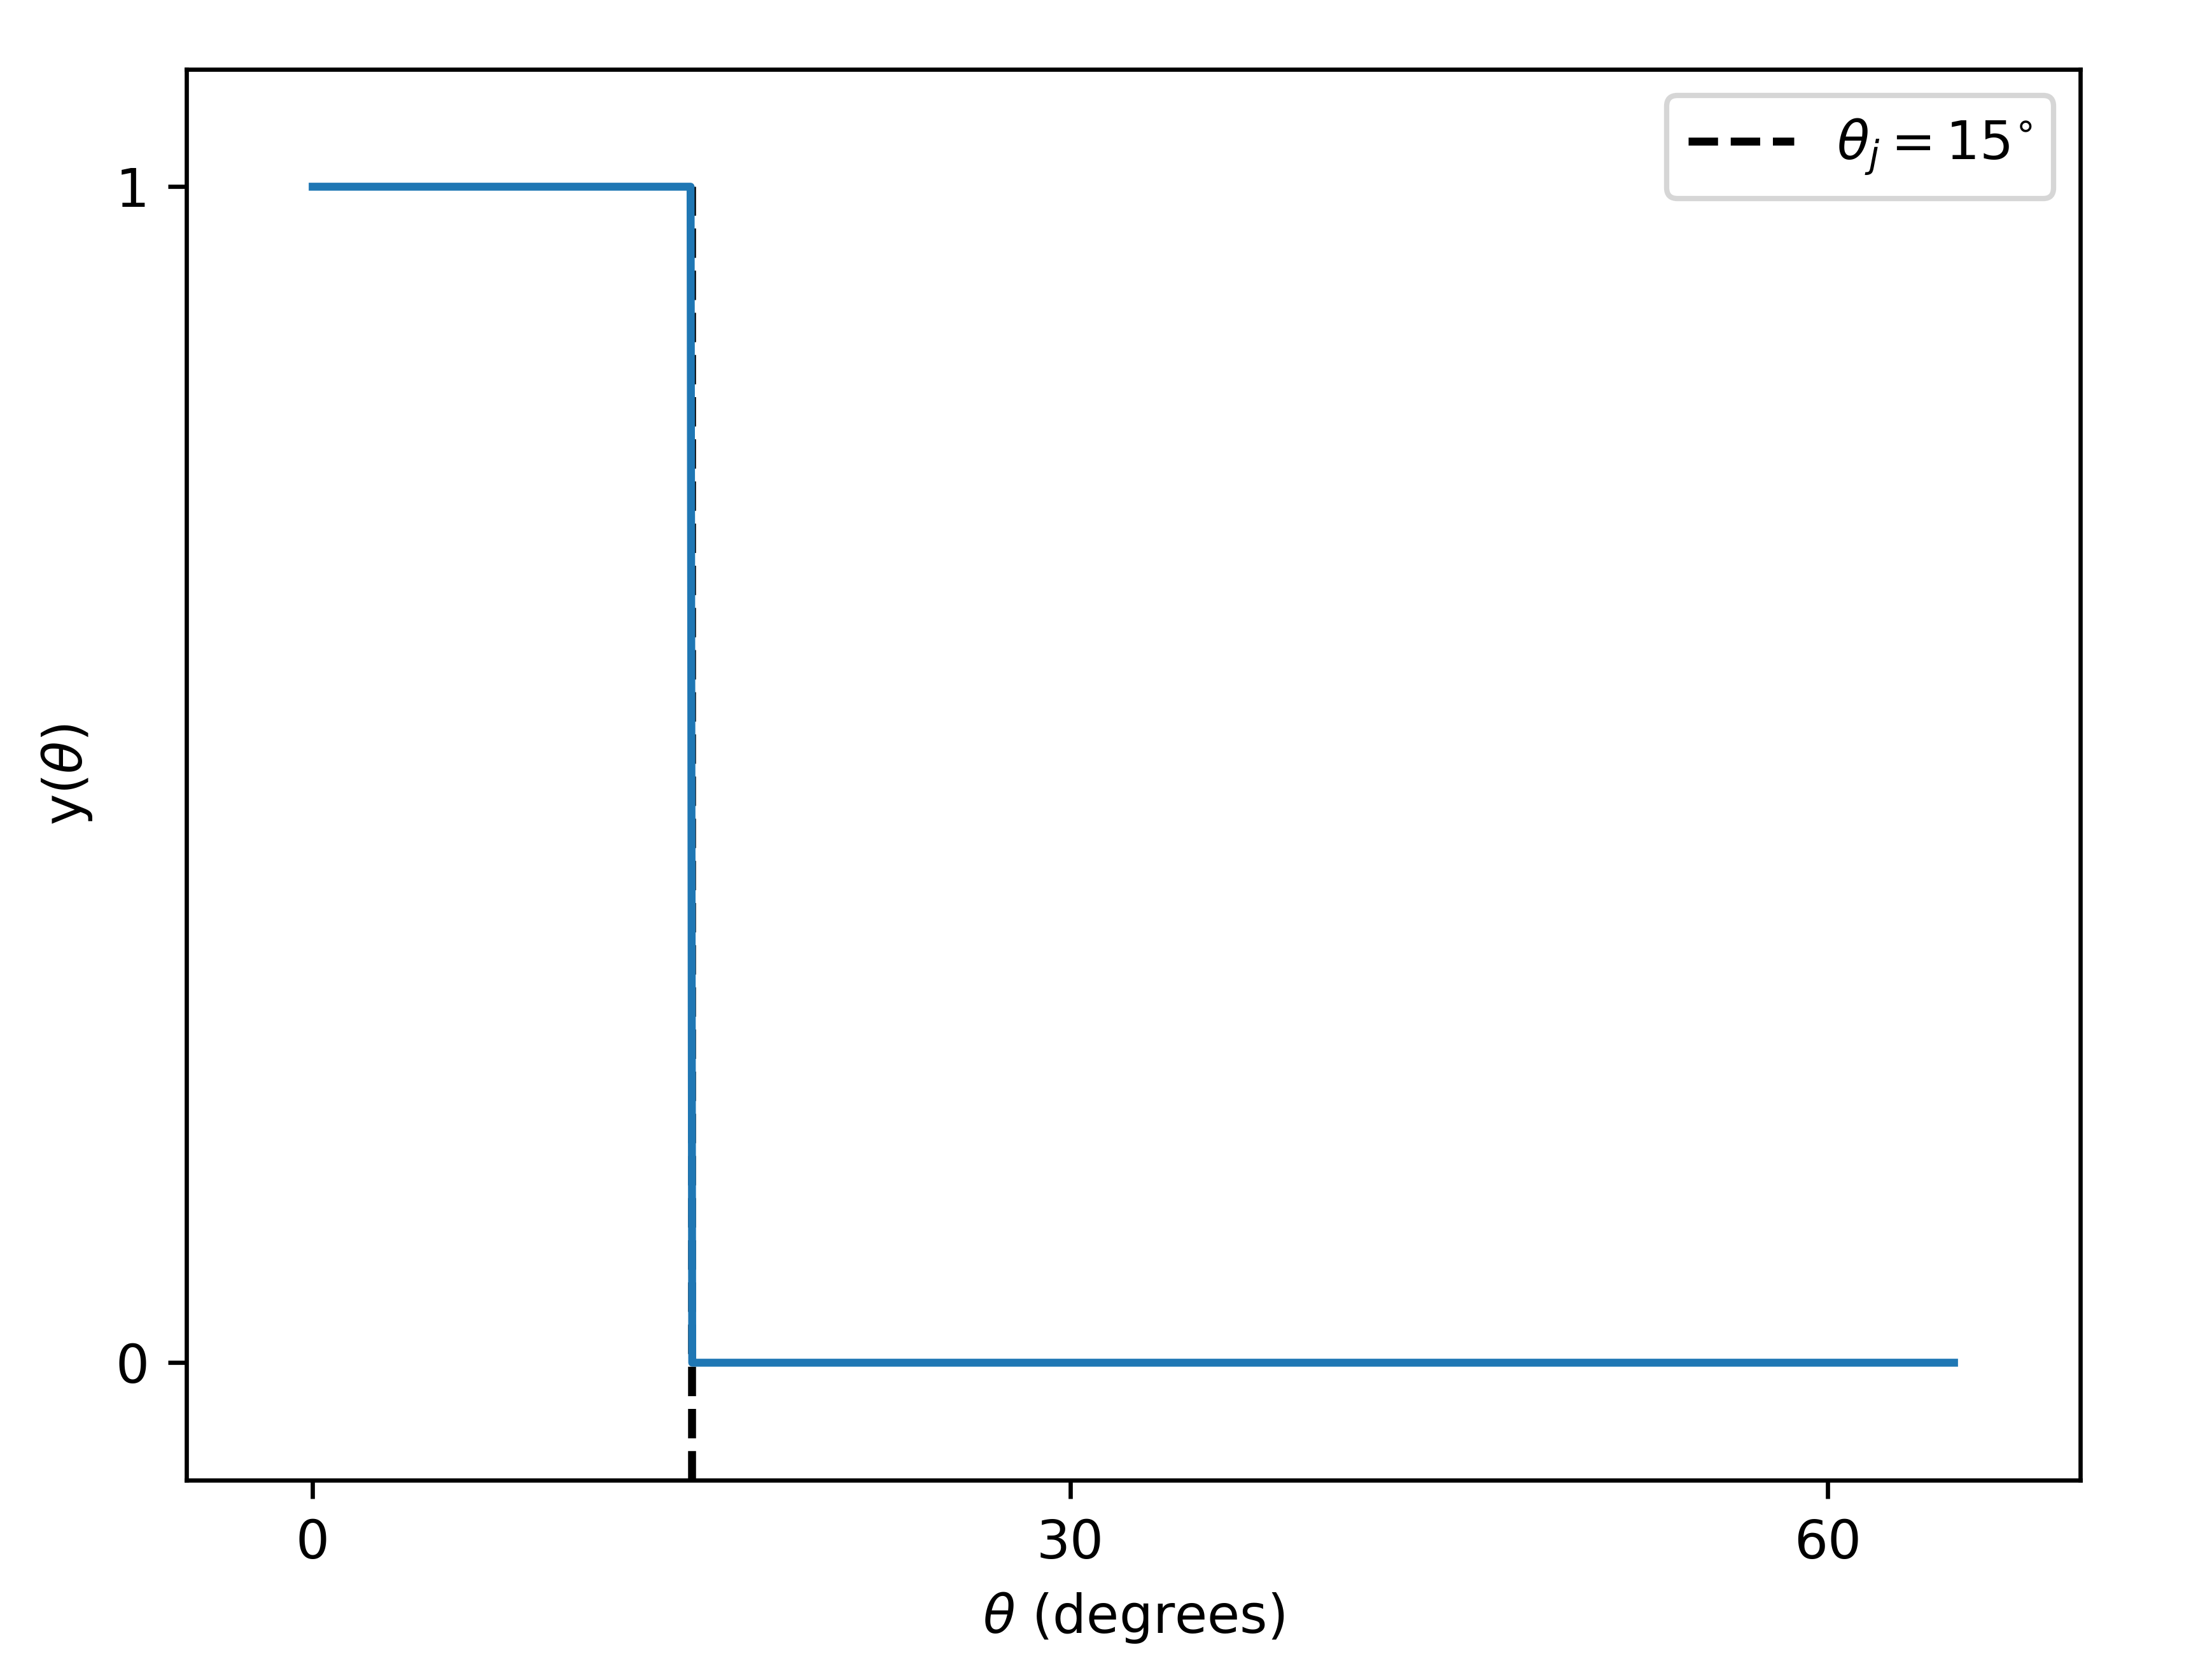
\includegraphics[width=10cm]{tophat}
        \caption[Tophat jet structure model]{
                    Functional form of the tophat jet structure model, as considered in
                    \cite{saleem_2020B}. The dashed line denotes the jet angle
                    $\theta_j = 15^{\circ}$.
             }
        \label{fig:tophat}
    \end{figure}

    \begin{figure}[H]
        \centering
        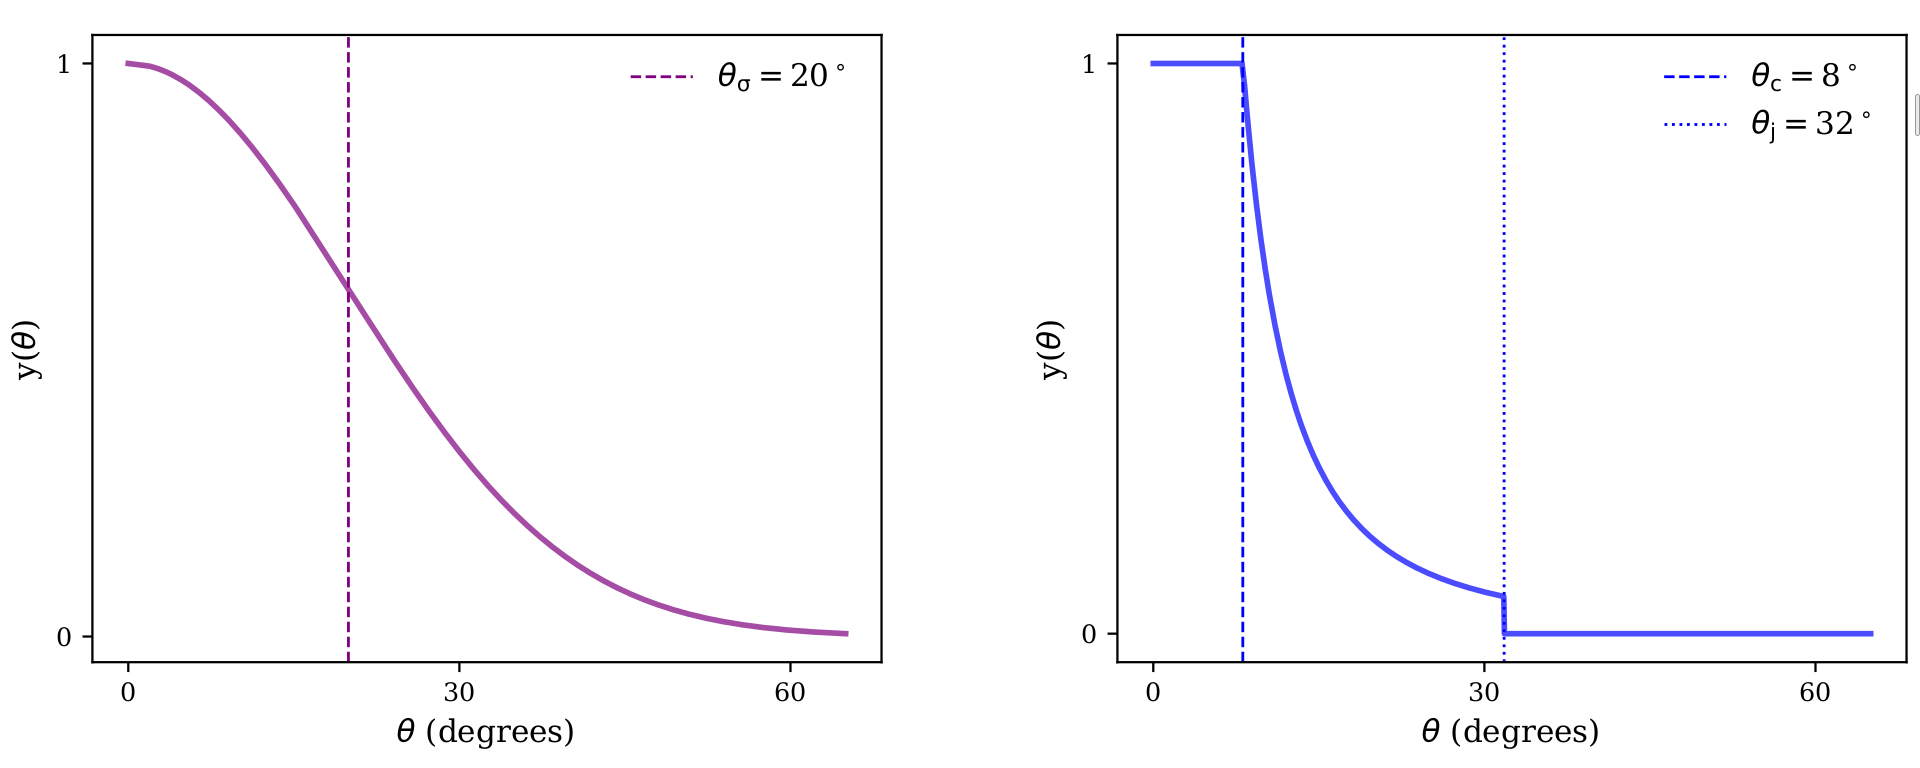
\includegraphics[width=\textwidth]{jet_models}
        \caption[Jet structures as in \cite{hayes_2020}]{
                    Functional forms of the jet structure models, as considered by
                    \cite{hayes_2020}. (Left) The gaussian jet structure with
                    a width $\theta_{\sigma} = 20^{\circ}$, also marked by the dashed
                    line. (Right) The power-law structure with a core angle $\theta_c =
                    8^\circ$ and a jet angle $\theta_j = 32^\circ$.
             }
        \label{fig:jet_models}
    \end{figure}

    In order to compute the observed structure given the intrinsic structure, following
    \cite{granot_2002} we start off by considering the emission profile of a
    point source moving at some angle with the observer, essentially rendering this
    scenario off-axis. This will affect the prompt jet emission, as well as the initial
    afterglow, and so warrants careful analysis.  Now, let the initial jet opening angle
    be $\theta_0$ and let the observer be at an angle $\theta_{obs}$. In general, for a
    point source moving at any angle $\theta$ with respect to the observer, the observed
    flux is given by :

    \begin{equation}
        \label{eq:1}
        F_{\nu} =
           \dfrac{L^{\prime}_{\nu^{\prime}}}{4 \pi d_L^2}
           \left( \dfrac{\nu}{\nu^\prime}\right)^3
                =
            \dfrac{1 + z}{4 \pi d_L^2}
            \dfrac{L^{\prime}_{\nu^{\prime}}}{\gamma^3 (1 - \beta \cos \theta)^3}
    \end{equation}

    Here, $L^{\prime}_{\nu^{\prime}}$ and $\nu^{\prime}$ are the jet comoving frame
    spectral luminosity and frequency, $d_L$ is the luminosity distance, $\gamma = (1 -
    \beta^2)^{-1/2}$ is the jet Lorentz factor. If $t$ and $\nu$ are the observed time
    and frequency  for an observer at $\theta$, and $t_0$ and $\nu_0$ are those for an
    observer on the axis, then:

    \begin{equation}
        \label{eq:2}
        \dfrac{t_0}{t} =
            \dfrac{\nu}{\nu_0}
                       =
            \dfrac{(1 - \beta)}{(1 - \beta \cos \theta)}
            \equiv a
            \approx \dfrac{1}{(1 + \gamma^2 \theta^2)}
    \end{equation}

    And finally putting Eq. \ref{eq:2} into Eq. \ref{eq:1} and expanding using a Taylor
    series approximation upto the leading order:

    \begin{equation}
        \label{eq:3}
        F_{\nu}(\theta_{obs}, t) = a^3 F_{\nu/a}(0, at)
    \end{equation}

    This gives us a handle on how to relate observed off-axis quantities to the on-axis
    ones. Furthermore, this enables us to go from an intrinsic structure to an observed
    one, which is what was required.

\section{Outflows from NSBH Mergers}\label{sec:nsbh}

    The main difference in the NSBH merger pathway to SGRBs, compared to the case of BNS
    mergers, is that though there is theoretical and simulational support for the
    launching of SGRB jets from the merger of a neutron star and a black hole of
    appropriate mass (see for example \cite{ruiz_2020}, \cite{shibata_2019},
    \cite{foucart_2020}), there has not been strong observational evidence for the same.
    In the first half of the third observing run of the LVC (also known as O3a), there
    have been several triggers which have been reportedly confident NSBH triggers.
    However, there were no counterpart EM signals picked up, which decreases the
    credibility of NSBH mergers as the progenitors of SGRBs.\\
    The electromagnetic component from NSBH mergers, is largely decided based on the
    amount of mass left post-merger, outside the horizon of the black hole. This decides
    how much matter participates in the subsequent processes, which may be the rapid
    neutron-capture process which gives rise to the kilonova signal or the magnetic
    field amplification process via the Magneto-Rotational Instability (MRI) which leads
    to a SGRB jet.\\
    Qualitatively, for a binary where the neutron star is treated as a test mass and the
    black hole's spin is aligned with the orbital angular momentum of the binary, the
    innermost-stable circular orbit radius $r_{ISCO}$ scales as $r_{ISCO} \sim
    f(\chi_{BH}) G M_{BH}/c^2$ (where f is a function ranging from 1 to 9, decreasing
    for increasing (prograde) spins; see \cite{bardeen_1972}) and the radius at which
    the tidal disruption of the neutron star occurs, $r_{dis}$ scales as $r_{dis} \sim k
    (M_{BH/M_{BNS}})^{1/3} R_{NS}$ (where k is a constant with a dependence on the black
    hole spin and the equation of state). Only requiring that $r_{dis} \gtrsim
    r_{ISCO}$, as a rough requirement for disruption to occur before the neutron star
    plunges into the black hole, leads to the conclusion that (a.) low-mass black holes
    (b.) larger NS radii (c.) higher prograde black hole spins favour disruption. This
    is seen from Fig. \ref{fig:nsbh_disruption_condition} as well. However, for actual
    quantitative results simulations need to be performed such the effect of the various
    components in the problem are correctly taken into account. As seen from the
    literature, wherein such general-relativistic magnetohydrodynamic simulations are
    carried out, the matter left over post-merger heavily depends on (for a summary, see
    Fig.  \ref{fig:rest_mass_fraction}):

    \begin{itemize}

        \item \textbf{The mass ratio of the system}. This is defined as $q = M_{BH} /
            M_{NS}$ so that $q > 1$ always. Fully general relativistic,
            magnetohydrodynamic simulations (such as \cite{ruiz_2020}) show that in
            cases where the  mass ratio is 3:1, regardless of the neutron spin, a
            collimated outflow is observed, whereas the same is not realised in cases
            where the mass ratio is 5:1 or higher.

        \item \textbf{The spin of the components of the system}. In geometrized units
            (where $G = c = 1$), these are prescribed in terms of $a_{BH} / M_{BH}$ or
            $a_{NS} / M_{NS}$, and whether these two spins align (prograde) or are
            anti-aligned (retrograde) decides whether the neutron star would be tidally
            disrupted, and hence participate in the processes mentioned previously, or
            not. Via simulations, it is seen that the more the prograde spin of the
            neutron star, the farther out the neutron star is tidally disrupted, albeit
            this is only observed for the case of q = 3:1 (comparing say, Figs.
            \ref{fig:nsbh_jet} and \ref{fig:nsbh_5to1}). Also, this leads to long tidal
            tails, which produces a baryon-loaded environment and thus the magnetic
            field of the tidally disrupted matter must overcome the baryon ram pressure
            to launch the jet. This process hence delays the launching of the jet.

    \end{itemize}

    Aside from the SGRB jet, which requires magnetic field amplification (via MRI) as
    well as thermal pair production (from the disk remnant) followed by the
    Blandford-Znajek process, there is a possibility that NSBH mergers can produce
    kilonovae signatures. For this, the dynamically ejected mass has to be between
    $10^{-4.5} - 10^{-2} (M_{NS}/1.4 M_{\odot}) M_{\odot}$ (see \cite{ruiz_2020} for
    more details), and this will lead to kilonovae potentially detectable by the Large
    Synoptic Survey Telescope (LSST).

    \begin{figure}[H]
        \centering
        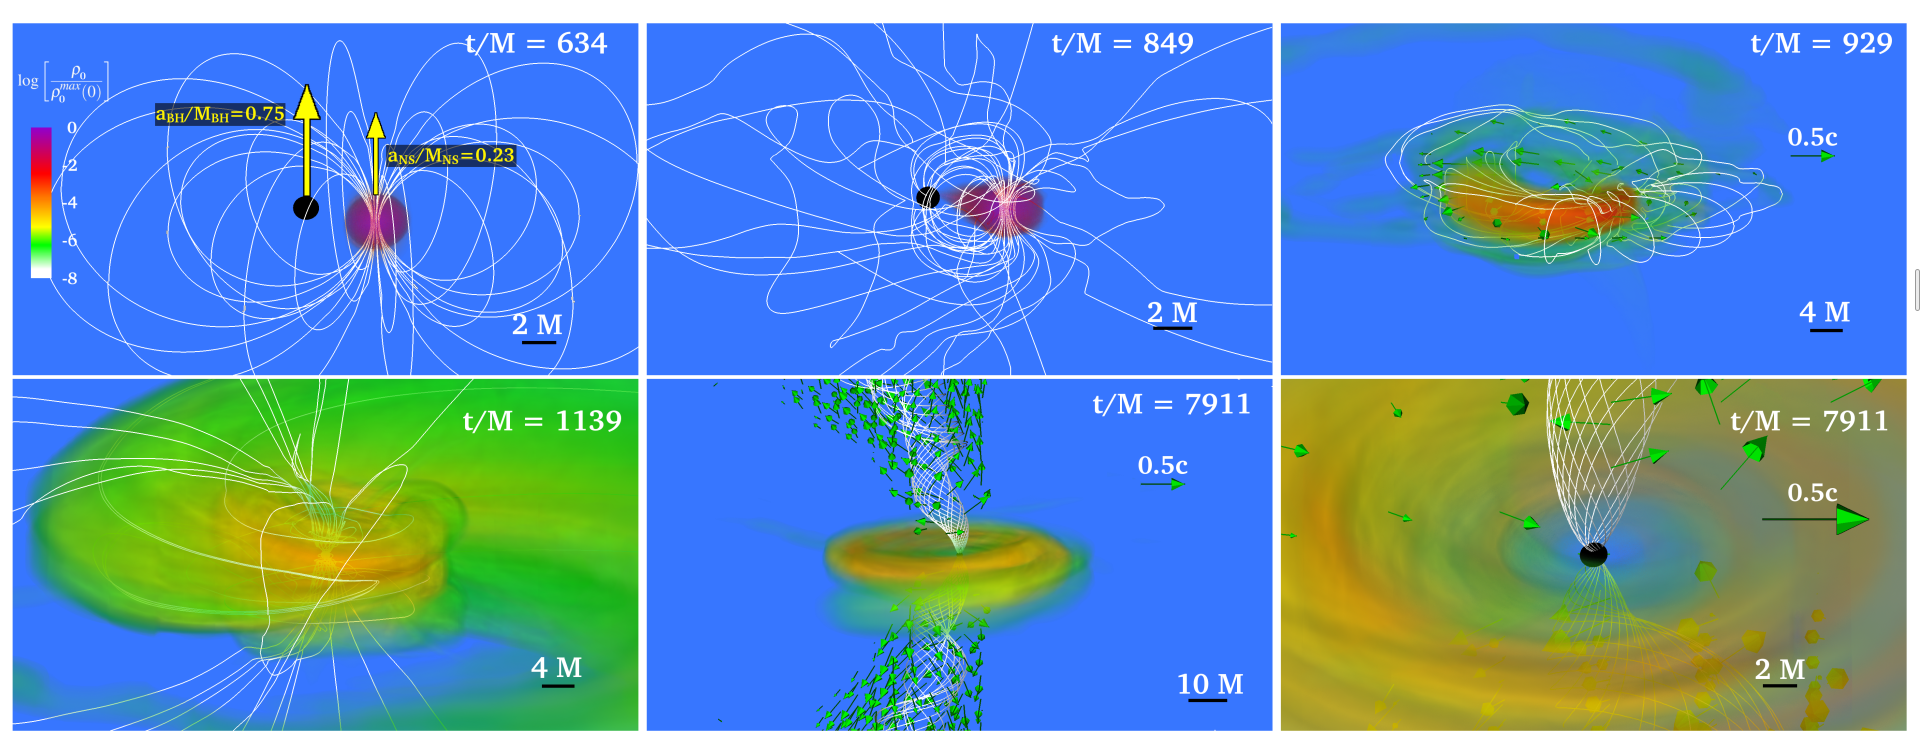
\includegraphics[width=\textwidth]{nsbh_jet}
        \caption[Tidal disruption of a NS in a 3:1 NSBH binary]{
                    Volume rendering of the rest mass density ($\rho_0$) (in log scale),
                    normalized to the NS maximum value $\rho_0 = 8.92 \times 10^{14}
                    (1.4 M_{\odot}/M_{NS})^2 \text{ g/cm}^3$, for particular times for a
                    magnetized neutron star, with q = 3:1 and a prograde NS spin of
                    0.23.  Top three panels highlight the inspiral and the tidal
                    disruption, whereas the bottom three panels highlight the appearance
                    of the magnetically-driven jet. White lines denote the magnetic
                    field, arrows denote the fluid velocity and the BH's apparent
                    horizon is the black sphere. Here M = $2.5 \times 10^{-2}
                    (M_{NS}/M_{1.4M_{\odot}}) \text{ ms} = 7.58
                    (M_{NS}/M_{1.4M_{\odot}}) \text{ km}$ (in geometrized units). From
                    \cite{ruiz_2020}.
             }
        \label{fig:nsbh_jet}
    \end{figure}

    \begin{figure}[H]
        \centering
        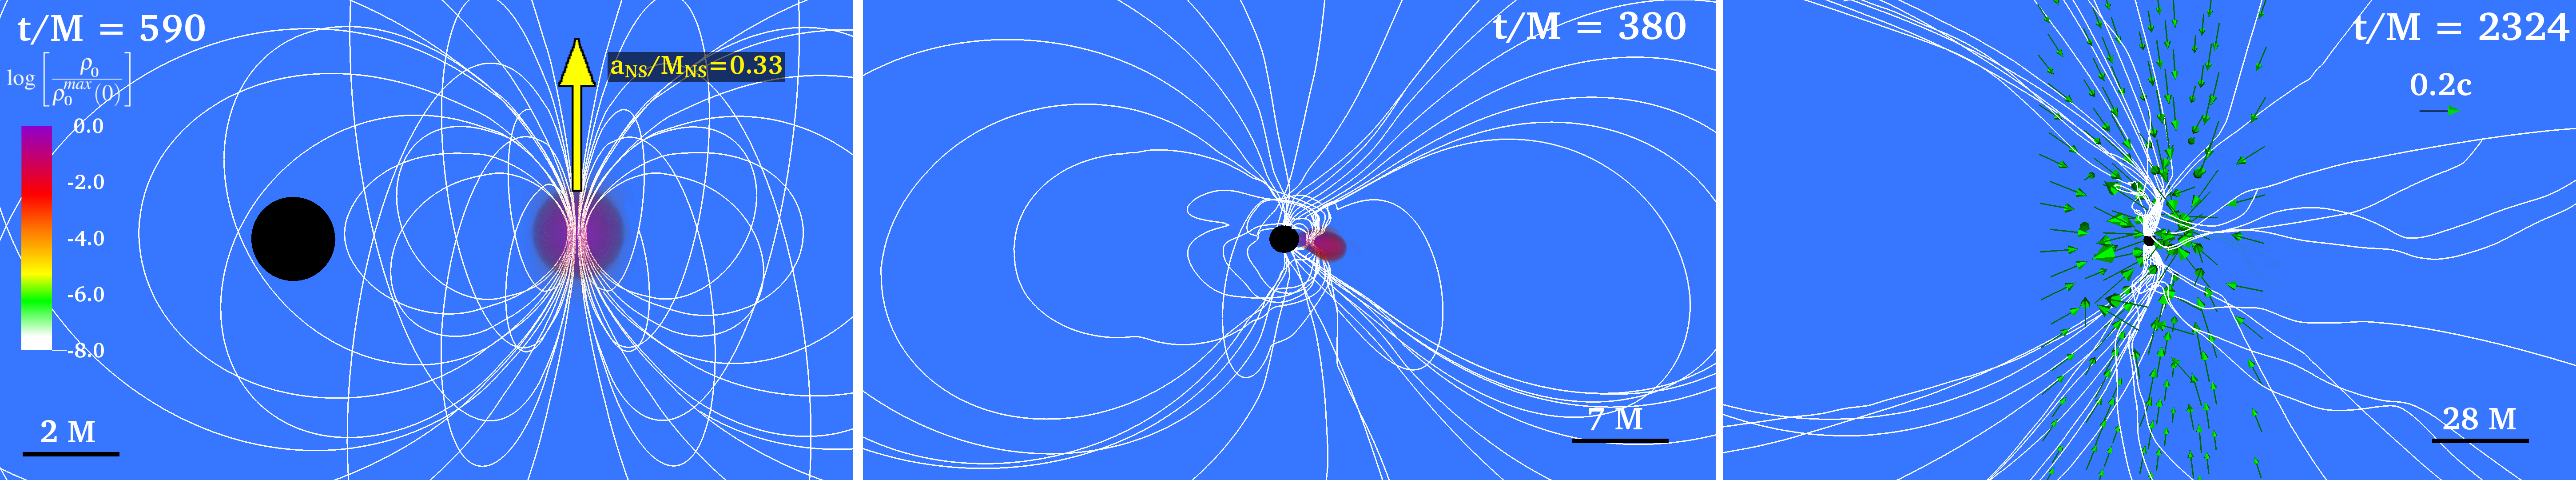
\includegraphics[width=\textwidth]{nsbh_5to1}
        \caption[Tidal disruption of a NS in a 5:1 NSBH binary]{
                    Similar to Fig. \ref{fig:nsbh_jet}, however with the NS spin being
                    0.33, the BH spin being 0 and q = 5:1. In this case, no strong
                    collimation of the magnetic field is observed from the merger
                    remnant, and so a magnetically-driven jet is also not observed.
                    From \cite{ruiz_2020}.
            }
        \label{fig:nsbh_5to1}
    \end{figure}

    \begin{figure}[H]
        \centering
        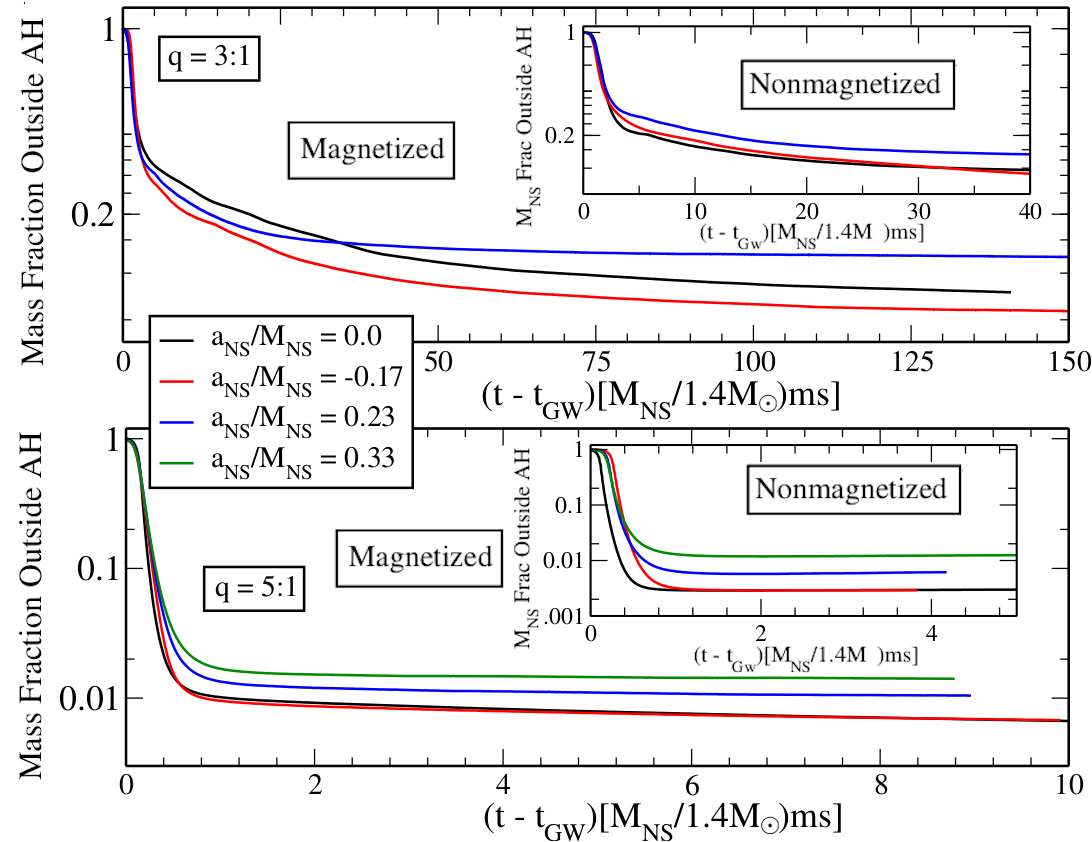
\includegraphics[width=11cm]{rest_mass_fraction}
        \caption[Rest mass outside black hole horizon, as a function of time]{
                    Fraction of rest-mass of the NS outside the apparent horizon of the
                    black hole as a function of coordinate time, for the various
                    configurations considered in \cite{ruiz_2020}. The inset figures
                    report the same for non-magnetized cases, and the coordinate time is
                    shifted such that the merger time coincides with 0.
            }
        \label{fig:rest_mass_fraction}
    \end{figure}

    \begin{figure}[H]
        \centering
        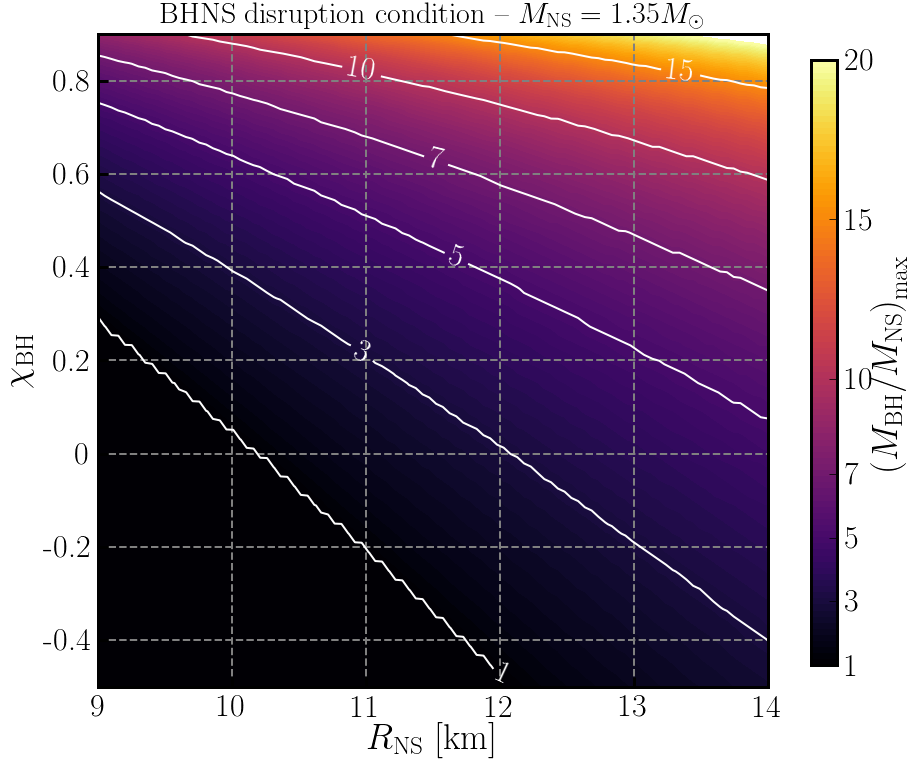
\includegraphics[width=9cm]{nsbh_disruption_condition}
        \caption[Disruption condition in a NSBH binary]{
                    Maximum value of the mass-ratio ($M_{BH}/M_{NS}$) for which a NSBH
                    system disrupts, as a function of the neutron star radius $R_{NS}$,
                    and the aligned component of the dimensionless black hole spin
                    $\chi_{BH}$, assuming $M_{NS} = 1.35 M_{\odot}$. Results for other
                    neutron star masses can be obtained by rescaling considering the
                    disruption condition at constant compaction $C_{NS} = GM_{NS}/R_{NS}
                    c^2$. From \cite{foucart_2020}.
            }
        \label{fig:nsbh_disruption_condition}
    \end{figure}

    \subsection{Modelling outflows from NSBH Mergers}\label{ssec:outflows-nsbh}

    As mentioned before, the outflows from NSBH mergers depend on the amount of mass
    left outside the event horizon post-merger. In the work done by \cite{foucart_2018},
    the authors consider a suite of 75 numerical relativity simulations of NSBH mergers
    over the parameter space $\mathcal{Q} \in [1, 7]$, $ \chi_{BH} \in [-0.5, 0.97]$,
    $\mathcal{C}_{NS} \in [0.13, 0.182]$\footnote{
        Here, $\mathcal{Q} = M_{BH}/M_{NS}$ is the mass-ratio, $\chi_{BH} =
        c|\mathbf{S}|/GM_{BH}^2$ is the effective spin of the black hole and $C_{NS} =
        GM_{NS}/R_{NS}c^2$ is the compactness of the neutron star.
    }
    and fit the results for the \textit{remnant mass} $M_{\mathrm{rem}}$ (sometimes also
    denoted as $M_{\mathrm{out}}$), as a function of the binary parameters (masses,
    spins of the components, tidal deformability of the neutron star etc). This fit is
    given as follows:

    \begin{equation}
        M_{\mathrm{out}} =
            M_{NS}^b \cdot
            \max \left( \alpha \dfrac{1-2\rho}{\eta^{1/3}} -
            \beta \hat{R}_{\mathrm{ISCO}} \dfrac{\rho}{\eta} + \gamma, 0 \right)^\delta
        \label{eq:m_out}
    \end{equation}
    where:

    \begin{itemize}

        \item The baryonic mass of the neutron star is given by the equation $$M_{NS}^b
            = M_{NS} \left(1 + \dfrac{0.6 C_{NS}}{1 + 0.5 C_{NS}} \right)$$

        \item The tidal deformability of the neutron star is given by $\Lambda_{NS}$ and
            $\rho = (15 \Lambda_{NS})^{-1/5}$. It is also related to the compactness of
            the neutron star via the C-Love relation (see \cite{yagi_2017}):
            \begin{equation}
                C_{NS} = \sum_{k=0}^{2} a_k (\ln \Lambda_{NS})^k
            \end{equation}
            where $a_0 = 0.360, a_1 = -0.0335, a_2 = 0.000705$.

        \item $\eta$ is the symmetric mass ratio, given by $ \eta =
            \dfrac{\mathcal{Q}}{(1 + \mathcal{Q})^2} $.

        \item $\hat{R}_{ISCO} = c^2 R_{ISCO} / GM_{BH}$ is the normalized ISCO radius
            for a spinning black hole, given in \cite{bardeen_1972} as :
            \begin{align}
                \hat{R}_{ISCO} &=
                    3 +
                    Z_2 -
                    \mathrm{sgn}(\chi_{BH}) \sqrt{(3 - Z_1)(3+Z_1 + 2Z_2)} \\
                \hookrightarrow Z_1 &=
                                1 +
                                (1 - \chi_{BH}^2)^{1/3}
                                [
                                    (1 + \chi_{BH})^{1/3} + (1 - \chi_{BH})^{1/3}
                                ] \nonumber \\
                \hookrightarrow Z_2 &=
                                \sqrt{3\chi_{BH}^2 +  Z_1^2} \nonumber
            \end{align}

        \item $(\alpha, \beta, \gamma, \delta) \equiv (0.308, 0.124, 0.283, 1.536)$ are
            the fit coefficients.

    \end{itemize}

    Similarly, \cite{kawaguchi_2016} fit to the results of 45 numerical relativity
    simulations over the parameter space $\mathcal{Q} \in [3,7]$, $\chi_{\mathrm{BH}}
    \in [0, 0.90]$, $C_{\mathrm{NS}} \in [0.138, 0.180]$. This fit produces a formula
    for the \textit{dynamic} mass $M_{\mathrm{dyn}}$, which is the unbound mass ejected
    at the time of disruption, in terms of the binary parameters. This fit is given as
    follows:

    \begin{multline}
        \dfrac{M_{dyn}}{M_{NS}^b} =
            \max \biggl\{
               a_1 Q^{n_1}(1 - 2C_{NS})C^{-1}_{NS} -
               a_2 Q^{n_2} \hat{R}_{ISCO}(\chi_{BH}) + \\
               a_3\left(1 - \dfrac{M_{NS}}{M^b_{NS}}\right) +
               a_4, 0
           \biggr\}
    \end{multline}
    where the symbols have their usual meanings, and additionally:

    \begin{align*}
        a_1 &= 4.464 \times 10^{-2} & a_2 &= 2.269 \times 10^{-3} \\
        a_3 &= 2.431 & a_4 &= -0.4159 \\
        n_1 &= 0.2497 & n_2 &= 1.352
    \end{align*}

    From these two quantities, we can derive the disc mass $M_{\mathrm{disc}}$ as :
    \begin{equation}
        M_{\mathrm{disc}} = \max\{M_{\mathrm{out}} - M_{\mathrm{dyn}}, 0\}
        \label{eq:disc_mass}
    \end{equation}
    However, due to the fact that these two fits are derived from simulations over
    different regions of the input parameter space, care must be taken while applying
    them together. This is to ensure that $M_{\mathrm{dyn}} \leq M_{\mathrm{out}}$
    always, so that the disc mass is non-negative. This validation is performed by
    considering the ratio $M_{\mathrm{out}} / M_{\mathrm{dyn}}$. Another constraint is
    imposed, which is motivated by the fact that NSBH simulations carried out by
    \cite{foucart_2019} in the near-equal mass ratio regime found an unbound component
    no more massive than roughly 30\% of the total remnant mass (note that one expects
    maximal tidal disruption in this regime, given a fast spinning black hole). Thus we
    set:

    \begin{equation}
        \label{eq:constraint}
        M_{\mathrm{dyn, max}} = f \cdot M_{\mathrm{rem}} = 0.3 \cdot M_{\mathrm{rem}}
    \end{equation}


    Additionally, the masses of the other wind ejecta, namely the neutrino-driven and
    viscosity-driven wind ejecta, are derived from that of the disc mass:
    \begin{align}
        \begin{split}
            M_{\mathrm{vis}} &=
                \xi_{\mathrm{vis}}M_{\mathrm{disc}} =
                    0.2M_{\mathrm{disc}} \\
            M_{\nu} &=
                \xi_{\nu}M_{\mathrm{disc}} =
                    0.01 M_{\mathrm{disc}}
        \end{split}
    \end{align}

    To model the SGRB jet, the procedure of \cite{zhu_2020} is followed. The
    kinetic energy of the jet is decided by the disc mass and the black hole spin as
    follows:
    \begin{equation}
        E_{\mathrm{K, jet}} =
            \epsilon(1 - \xi_{\mathrm{vis}} - \xi_{\nu})
            M_{\mathrm{disc}} c^2 \Omega_H^2 f(\Omega_H)
        \label{eq:e_kin_jet}
    \end{equation}
    where:

    \begin{itemize}

        \item The dimensionless angular velocity at the horizon of the black hole is
            given by:
            \begin{equation}
                \Omega_H = \dfrac{\chi_{BH}}{2(1 + \sqrt{1 + \chi_{BH}^2}}
            \end{equation}

        \item $f(\Omega_H)$ is a high-spin correction factor given by:
            \begin{equation}
               f(\Omega_H) = 1 + 1.38\Omega_H^2 - 9.2 \Omega_H^4
               \label{eq:Omega_h}
            \end{equation}
        \item $\epsilon$ is a fudge factor which depends on the large-scale geometry of
            the magnetic field, disc aspect ratio and the ratio of the magnetic field
            energy density to disc pressure at saturation.\\ In order to set it to a
            definite value, it is noted that the maximum disc mass cannot exceed the
            total NS baryonic mass i.e. $M_{\mathrm{disc}} \lesssim 2M_\odot$. Also, the
            spin-dependent factor $\Omega_H^2f(\Omega_H)$ cannot exceed 0.2 (since
            $\chi_{BH} \in [-1, 1]$). Furthermore, the most energetic of SGRBs has had a
            $E_{\gamma, \mathrm{iso}} \sim 7.4 \times 10^{52}$ erg, and if one assumes a
            10\% conversion efficiency of kinetic to gamma-ray energy alongwith a
            typical jet opening angle of 5$^{\circ}$, this corresponds to a kinetic
            energy of $E_{\mathrm{K, jet}} \sim 3 \times 10^{52}$ erg.\\
            Based on this, once can calculate $\boxed{\epsilon \approx 0.015}$.

    \end{itemize}

    Using this we can define the structure of the SGRB jet, given by the following
    equations:

    \begin{equation}
        \dfrac{dE(\theta)}{d\Omega} =
            \dfrac{E_{\mathrm{k, jet}}}{\pi \theta_{\mathrm{c, E}}^2}
            e^{-(\theta/\theta_{\mathrm{c, E}})^2}
        \label{eq:dE_dOmega}
    \end{equation}

    \begin{equation}
        \Gamma(\theta) = (\Gamma_c - 1)e^{-(\theta/\theta_{\mathrm{c, E}})^2} + 1
    \end{equation}

    \begin{equation}
        E_{\mathrm{iso}}(\theta_v) =
            \eta \int \dfrac{\delta^3}{\Gamma} \dfrac{dE}{d\Omega} d\Omega
        \label{eq:eiso}
    \end{equation}
    where:

    \begin{itemize}

        \item $\Gamma_c = 100, \theta_{\mathrm{c, E}} = 0.1, \theta_{\mathrm{c}, \Gamma}
            = 0.2$.  See \cite{salafia_2015} and \cite{barbieri_2019}.

        \item $\eta$ is the conversion efficiency of gamma-ray energy to kinetic energy,
            which is traditionally taken to be 10\%.

        \item $\delta$ is the Doppler factor, given by $$\delta = \dfrac{1}{\Gamma[1 -
            \beta \cos \alpha_v]}$$ where $\alpha_v$ is the angle between the jet
            element at $(\theta, \phi)$ and the observer's direction.
    \end{itemize}

\section{NS mergers in GW regime}

    Consider any astrophysical source emitting gravitational waves, which come in two
    polarizations, namely the \emph{plus} $h_{+}(t; \mathbf{\Theta}_{GW})$ and the
    \emph{cross} $h_{\times}(t; \mathbf{\Theta}_{GW})$ polarizations. Here
    $\mathbf{\Theta}_{GW}$ is the parameter vector, and is typically $\{m_1, m_2,
    \mathbf{\chi}_1, \mathbf{\chi}_2, D_L, \iota, t_c, \phi_c\}$ which are the component
    masses, component spins, the binary's luminosity distance, the inclination angle
    of the orbital plane with respect to the line of sight, and two constants of
    integration: the time and phase of coalescence.\\
    A detector's response is recorded as the GW strain such waveforms produce, but in
    the frequency domain and so the input waveforms are Fourier transformed before
    processing. Also the detector's antenna patterns (sensitivity as a function of the
    source location on the sky) and location phase factor (effect of the earth's
    rotation) play a role in the response. Thus, the detector response to these
    gravitational waves is of the form:
    \begin{equation}
        H(f; \mathbf{\Theta}) =
            F_{lp}(f; \alpha, \delta) \cdot
            [
                H_{+}(f; \mathbf{\Theta}_{GW}) F_{+}(f; \alpha, \delta, \psi) +
                H_{\times}(f; \mathbf{\Theta}_{GW}) F_{\times}(f; \alpha, \delta, \psi)
            ]
    \end{equation}
    where $F_{lp}$ is the location phase factor as a function of the frequency and the
    source RA and declination, $H_{+/\times}$ are the frequency domain waveforms, and
    $F_{+/\times}$ are the detector antenna patterns for each polarization. Also
    $\mathbf{\Theta} = \{\mathbf{\Theta}_{GW}, \alpha, \delta, \psi\}$.\\
    The sensitivity of a detector is given by the detector's noise $n(t)$ and its
    autocorrelation $\kappa = \overline{n(t_1)n(t_2)}$. Usually, the noise is assumed to
    be stationary, zero-mean and Gaussian. Thus, one can define the one-sided power
    spectral density $S_n(f)$ as the Fourier transform of the autocorrelation.\\
    From this, one can define the `overlap' between two GW signals (for eg.: the
    detector responses for two different waveforms) using the noise-weighted scalar
    product:
    \begin{equation}
        \langle H, G \rangle =
            2 \int_{0}^{\infty} \dfrac{H(f)G^{\ast}(f) + H^{\ast}(f)G(f)}{S_n(f)} df
    \end{equation}
    And using this definition of the scalar product, the signal-to-noise ratio is
    defined as :
    \begin{equation}
        \rho^2 =
            \langle H, H \rangle =
                4 \int_0^\infty \dfrac{|H(f)|^2}{S_n(f)} df
    \end{equation}
    Now, since the noise $n(t) = s(t) - h(t)$ is assumed to a zero-mean Gaussian, its
    Fourier transform also behaves the same way, and thus the probability of noise can
    be written down as :
    \begin{equation}
        \label{eq:probability}
        p(\mathbf{\Theta}) =
            p^0(\mathbf{\Theta})
            e^{
                -\frac{1}{2}
                \langle S - H(\mathbf{\Theta}), S - H(\mathbf{\Theta}) \rangle
            }
    \end{equation}
    where $p^0$ is the prior on the parameter vector of the detector response. Assuming
    that an event signal S has a high SNR, the value of $\mathbf{\Theta}$ at peak
    probability is a good estimate of the true value $\mathbf{\Theta}^{\ast}$.
    Additionally peak probability occurs when the exponential $E = \langle S - H, S - H
    \rangle$ is the largest. Expanding it around the maximum value:
    \begin{equation}
        E(\mathbf{\Theta}) =
            E(\mathbf{\Theta}^{\ast}) +
            \dfrac{1}{2}
            \dfrac{\partial^2 E(\mathbf{\Theta})}{\partial \Theta_i \partial \Theta_j}
            \bigg\rvert_{\mathbf{\Theta} =
                \mathbf{\Theta}^{\ast}}
                \Delta\Theta_i \Delta\Theta_j +
                \cdots
    \end{equation}
    where $\Delta \Theta_i = \Theta_i - \Theta_i^\ast$. The Hessian given by:
    \begin{equation}
        \dfrac{\partial^2 E(\mathbf{\Theta})}{\partial \Theta_i \partial \Theta_j} =
            2 \langle
                  \partial_{\Theta_i} H(\mathbf{\Theta}),
                  \partial_{\Theta_j} H(\mathbf{\Theta})
              \rangle +
              \langle
                  \partial_{\Theta_i} \partial_{\Theta_j} H(\mathbf{\Theta}),
                  N
              \rangle
    \end{equation}
    can be simplified for large SNR, where second-order differentials become negligible.
    This leads to the definition of the Fisher Information Matrix $\Gamma$:
    \begin{equation}
        \Gamma_{ij} =
            \langle
                \partial_{\Theta_i} H(\mathbf{\Theta}),
                \partial_{\Theta_j} H(\mathbf{\Theta})
            \rangle
    \end{equation}
    And hence, Eqn. \ref{eq:probability} becomes:
    \begin{equation}
        p(\mathbf{\Theta}) \sim
            \exp\left(
                         -\dfrac{1}{2}
                          \Gamma_{ij}
                          \Delta\Theta_i
                          \Delta\Theta_j
                \right)
    \end{equation}
    which implies that the assumption of Gaussian noise helps associate the FIM to the
    inverse of the covariance matrix $\Sigma \equiv \Gamma^{-1}$. This also means that
    the diagonal and off-diagonal elements of $\Gamma^{-1}$ denote the variances and
    covariances of the parameters, respectively, with 1$\sigma$ estimates of the error
    are given as $\sigma_{\Theta_i} = \sqrt{\Sigma_{ii}}$.\\
    This Fisher Information Matrix (FIM) formalism\footnote{
        Sometimes also referred to as the Fisher Information Formalism (FIF), in which
        case the Fisher information is not a matrix but is instead the variance of the
        partial derivative with respect to the parameter vector, of the natural
        logarithm of the likelihood function for the random variable whose parameters
        are to be estimated.
    } is a method of rapid GW data analysis, which approaches the accuracy of
    traditional Bayesian parameter estimation for events with large SNR.\\
    \textbf{GWBENCH} (see \cite{borhanian_2020}) is a GW benchmarking tool, which can
    compute the Fisher matrix for a particular NS merger, given the network
    configuration and binary parameters. In this way, it enables rapid calculations to
    benchmark detector upgrades as well as forecast the confidence with which parameters
    may be estimated for the NS mergers in question.\\

\section{Summary}

    NS mergers can present an ideal testing environment for physical theories under
    extreme gravity, and by observing them in both the EM and GW windows, current
    theories can be better understood and refined. Several questions also remain about
    the exact mechanisms which power the outflows from these NS mergers.\\
    In this report, we focus mainly on SGRB jets from NSBH mergers and perform
    population synthesis studies to infer the conditions for and implications of
    observing a SGRB jet from NSBH mergers.
  % Introduction
                      % DONE: Fix to make appropriate

    \chapter{Population Synthesis}\label{ch:synthesis}
    In order to derive meaningful conclusions about the outflows from NS mergers, given
    the models described in \ref{ch:introduction}, it was necessary to carry out
    population synthesis studies. In these, population models which are physically or
    observationally motivated are taken from the literature and used to compute the
    statistical properties of the outflows from NS mergers created with these
    properties. If no confident or relevant model exists in literature, physically
    motivated ans\"{a}tze are used (see for example, \S\S\ref{sub:spin-dists}).\\
    In each study which uses (slightly) different population models, 10$^5$ samples were
    drawn from the relevant parameter distributions. Using these as inputs the expected
    outflows were calculated using the fit formulae described in
    \ref{ch:introduction}.\\
    In this chapter, the various population models are briefly described along with
    their pertinence. Furthermore, preliminary checks for the population synthesis code
    are also discussed, which help verify the consistency of the code with theoretical
    results.

\section{Black Hole Population Models}\label{sec:bh_pop}

    \subsection{Mass, $M_{BH}$}
        The masses of the black holes was sampled from the \textsc{truncated} mass
        distribution from \cite{abbott_2020B}. The distribution `produces' black holes
        with masses between 3--100 M$_\odot$ (as can be seen from Fig.
        \ref{fig:bh_mass_gwtc2}).  However, NS binaries with extremely massive ($M_{BH}
        > 20 M_\odot$) black holes will not produce any appreciable EM emission due to
        the NS companion plunging into the black hole directly without significant tidal
        disruption. For this reason the population synthesis code imposes an upper limit
        to the black hole masses sampled.

        \begin{figure}[H]
            \centering
            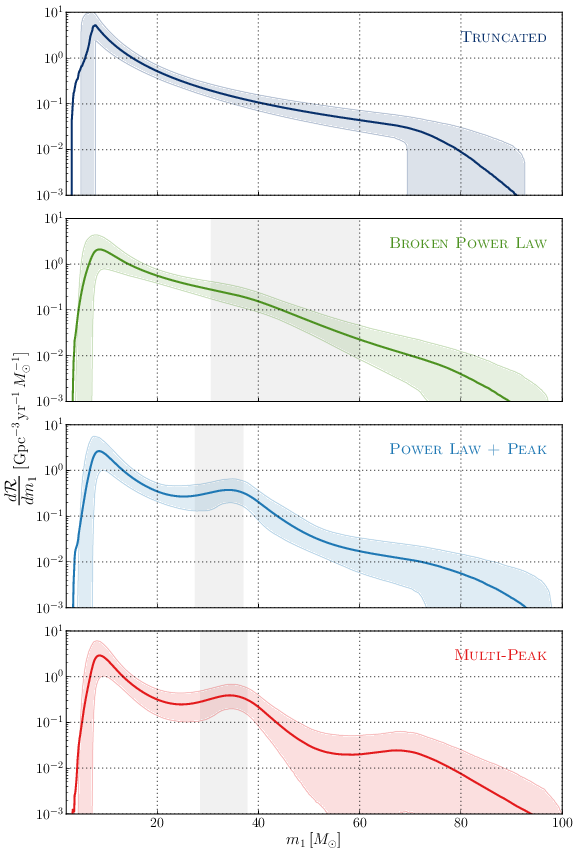
\includegraphics[width=0.9\linewidth]{bh_mass_gwtc2}
            \caption[Black hole mass distributions from GWTC-2]{
                Black Hole Mass Distributions from \cite{abbott_2020B}. In the current
                study the \textsc{truncated} mass distribution with an upper limit at 20
                M$_\odot$, since more massive black holes would not produce significant
                EM emission when in a merging NSBH binary.
            }
            \label{fig:bh_mass_gwtc2}
        \end{figure}

        \begin{figure}[H]
            \centering
            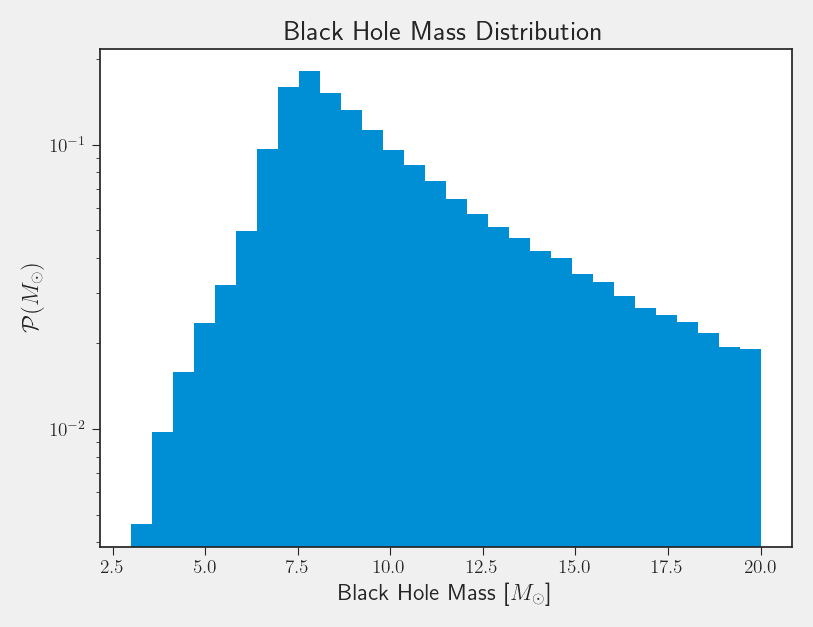
\includegraphics[width=0.8\linewidth]{bh_mass}
            \caption[Black hole mass distribution with upper limit]{
                Black hole mass distribution as used in the current report, with an
                upper limit of 20 M$_\odot$.
            }
            \label{fig:bh_mass}
        \end{figure}

    \subsection{Spin, $\chi_{BH}$}\label{sub:spin-dists}
        The spins of the black holes are sampled from the \textsc{default} distribution
        given in \cite{abbott_2020B}. This distribution is essentially a Beta
        distribution , which ensures that the spin parameters sampled from this
        distribution remain within [0, 1).\\
        However, since there have been no confident NSBH merger detections in the GW
        regime, this distribution is largely derived from looking at BBH mergers, and so
        may not represent the true spin distribution of a black hole in a NSBH binary.
        To circumvent this, the following ans\"{a}tze are used to probe the effect of
        the spin distribution on the EM outflows:

        \begin{figure}[H]
            \centering
            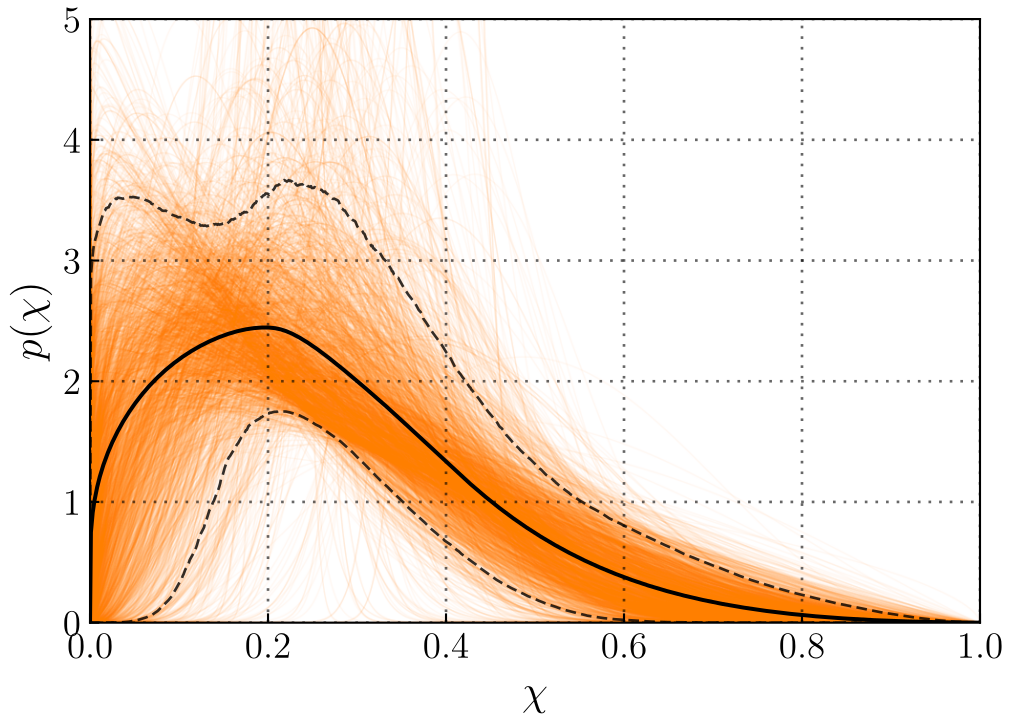
\includegraphics[width=0.8\linewidth]{bh_spin_gwtc2}
            \caption[Black hole spin distribution from GWTC-2]{
                Beta distribution for the  black hole spin from \cite{abbott_2020B}.
                Here the light traces are samples from the posterior distribution,
                whereas the solid black line is the posterior probability distribution
                for $\chi_{BH}$. Dashed black lines mark the 90\% quantiles for the
                same.
            }
            \label{fig:bh_spin_gwtc2}
        \end{figure}


        \begin{itemize}

            \item Uniform spin distribution: here $\chi_{BH} \sim \mathcal{U}(0, 1)$.
                Note also that this distribution will have a higher number of high spin
                samples as compared to the \textsc{default} distribution considered
                above.

                \begin{figure}[H]
                    \centering
                    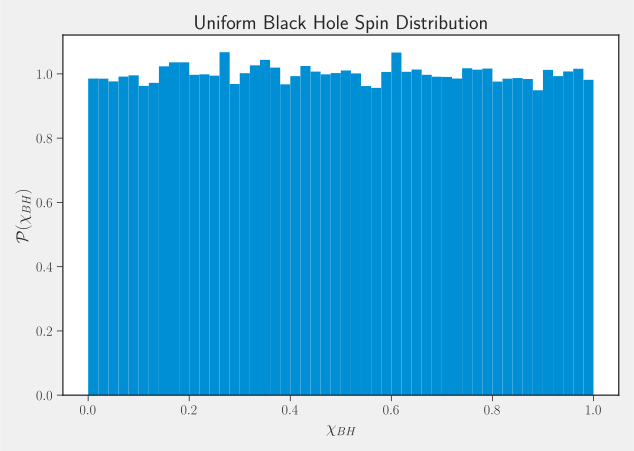
\includegraphics[width=0.7\linewidth]{unif_dist}
                    \caption[Uniform Black Hole Spin Distribution]{
                        A realisation of the uniform black hole spin distribution
                        considered here.
                    }
                    \label{fig:unif_dist}
                \end{figure}

            \item Gaussian spin distribution: here $\chi_{BH} \sim \mathcal{N}(\mu,
                \sigma)$, but samples outside of [0, 1) are not considered. For
                simplicity and to cover a representative sample of the possible
                distributions, samples were taken from $\mathcal{N}(0.2, 0.2)$,
                $\mathcal{N}(0.5, 0.2)$ and $\mathcal{N}(0.7, 0.2)$. These represent
                distributions concentrated around low, medium and high spins
                respectively.

                \begin{figure}[H]
                    \centering
                    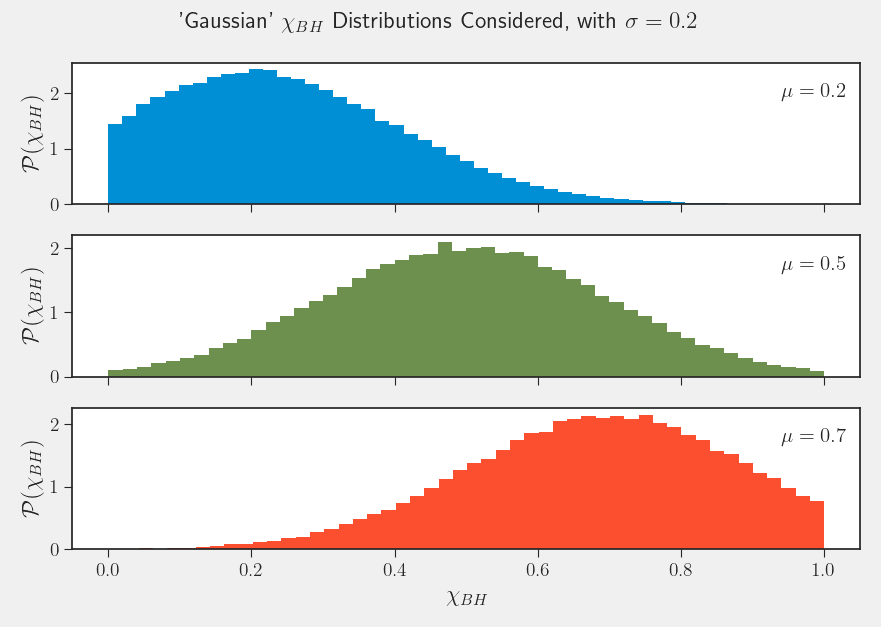
\includegraphics[width=0.8\linewidth]{gauss_dists}
                    \caption[Gaussian Black Hole Spin Distributions]{
                        Realisations of the various `Gaussian' black hole spin
                        distributions considered here.
                    }
                    \label{fig:gauss_dists}
                \end{figure}

        \end{itemize}


\section{Neutron Star Population Models}\label{sec:ns_pop}

    In order to reduce the number of variables in the problem, the masses of all neutron
    stars in the population was set to 1.4 M$_\odot$. This value corresponds to the
    median neutron star mass as inferred from GW170817 (see \cite{abbott_2018}). Also,
    the spins of all neutron stars was set to 0, since it is assumed that sufficient
    amount of time would have passed between the formation of the binary and merger,
    allowing for the neutron star to spin down such that $\chi_{NS} \sim 0$.\\
    Additionally, the tidal deformability of the neutron stars was set using the C-love
    relation (see \cite{yagi_2017}). First, the radii of the neutron stars were set to
    11 km, which is the median neutron star radius inferred for GW170817. Then, the
    compactness of the neutron stars, $C_{NS}$ was computed using the relation :

    \begin{equation}
        C_{NS} = \dfrac{G M_{NS}}{R_{NS} c^2}
    \end{equation}

    where $M_{NS}$, $R_{NS}$ are the mass and radius of the neutron star, G is the
    universal gravitational constant and c is the speed of light.  Finally, the tidal
    deformability is computed by solving the C-Love relation :

    \begin{equation}
        C_{NS} = \sum_{k=0}^{2} a_k (\ln \Lambda_{NS})^k
    \end{equation}

    where $\Lambda_{NS}$ is the tidal deformability of the neutron star, and $a_k$ are
    the fit coefficients as given in \cite{yagi_2017}.

\section{Spatial Distribution and Orientation of events}\label{sec:space_dist}

    \subsection{Constant comoving volume distribution}

        The events whose component mass and spin distributions were described in
        \ref{sec:bh_pop}-\ref{sec:ns_pop} are distributed in 3D space such that their
        number density is constant in comoving volume.\\
        For this, firstly the latitudinal ($\theta$) and longitudinal ($\phi$) angles
        are sampled such that $\cos \theta \sim \mathcal{U}(-1, 1)$ and $\phi \in
        \mathcal{U}(0, 2\pi)$, i.e. they are sampled such that they are uniform on a
        unit sphere. As for the comoving distance distribution $\mathcal{P}(D_c)$,
        consider the probability of an event lying in an infinitesimal shell of width
        d$D_c$ at a comoving distance $D_c$.  Then it can be seen that:
        \begin{equation}
            \mathcal{P}(D_c) dD_c \propto D_c^2 dD_c \Rightarrow
                \boxed{\mathcal{P}(D_c) = \alpha D_c^2}
        \end{equation}
        where $\alpha$ is the constant of proportionality. In the local universe, it can
        be safely assumed that $D_c \approx D_L$, where the latter is the luminosity
        distance.  However, from the fact that the GW SNR $\rho \propto D_L^{-1}$ it can
        also be seen that:

        \begin{align}
            \mathcal{P}(\rho) &= \mathcal{P}(D_L)
                                  \Big \lvert \dfrac{dD_L}{d\rho} \Big \rvert \\
                              &= \mathcal{P}({D_c})
                                  \Big \lvert \dfrac{dD_c}{d\rho} \Big \rvert \\
                              &\propto \dfrac{1}{\rho^2} \dfrac{1}{\rho^2}
                                  = \dfrac{1}{\rho^4} \nonumber\\
            \Rightarrow \mathcal{P} (\rho) &= \dfrac{\beta}{\rho^4}
        \end{align}

        Once the SNR detection threshold\footnote{
            This is defined such that any event with a GW network SNR greater than the
            detection threshold will be considered a detection.
        } ($\rho_{th}$) is set, the normalization constants can be computed as follows:

        \begin{align}
            \int_0^{D_{c, max}}
                \mathcal{P}(D_c) dD_c &= \int_0^{D_{L, max}} \mathcal{P}(D_L) dD_L \\
                                      &= \int_\infty^{\rho_{th}} \mathcal{P}(\rho)
                                          d\rho \\
                                      &= 1
        \end{align}

        This gives:

        \begin{align}
            \label{eq:lum_dist}
            \mathcal{P}(D_L) = 3 \dfrac{D_L^2}{D_{L, max}}
                                 \Leftrightarrow
            \mathcal{P}(\rho) = 3 \dfrac{\rho_{th}^3}{\rho^4}
        \end{align}

        where $D_{L, max}$ is the luminosity distance corresponding to the detection
        threshold. As an example, for the Advanced LIGO/VIRGO configuration and a SNR
        threshold of 10, $D_{L, max} \approx 1123$ Mpc.\\
        Using Eq.\ref{eq:lum_dist}, samples are drawn from the luminosity distance
        distribution and using the previous samples for $\theta$ and $\phi$, events are
        distributed in 3D space such that the number density of events is constant in
        the comoving volume.

    \subsection{Orientation of Events}\label{sub:orientation_of_events}

        The orientation of NSBH binaries with respect to the line-of-sight is prescribed
        using the inclination angle, $\iota$ and the polarization angle of the incoming
        GW signal, $\psi$. These are distributed for the population such that $\cos\iota
        \sim \mathcal{U}(-1, 1)$ and $\psi \sim \mathcal{U}(0, 2\pi)$, from which
        samples are drawn for individual events.

\section{Validation of Population Synthesis Code}\label{sec:popsyn_validation}

    With the population models for the binary component parameters as described in the
    previous section, 10$^5$ samples are drawn from each model to generate a population.
    These populations will majorly differ in the black hole spin distribution and are
    thus distinguished by that very factor.\\
    Given these populations, several checks were carried out to confirm the consistency
    of the underlying models and the population generated, with the use of (both EM and
    GW) theoretical results. The rationale behind these checks and the results are given
    in the following sections.

    \subsection{GW Checks}\label{sub:gw_checks}

        Firstly, for the samples generated, the optimal GW SNR corresponding to the
        binary parameter combinations was computed. This was done by using the
        restricted post-Newtonian (PN) waveform (RWF; see \cite{cutler_1994}) as the GW
        template for the expected GW strain signal from an actual merger event. For this
        case, the template is given using the frequency domain representation:

        \begin{equation}
            \tilde{h}(f) = \mathcal{A}f^{-7/6}e^{i\phi(f)}
            \label{eq:rwf}
        \end{equation}

        where $\mathcal{A} = \sqrt{5/96}\pi^{-2/3} \mathcal{M}$ is the amplitude,
        $\mathcal{M} = M \eta^{5/3}$ is the chirp mass, $M$ is the total mass, $\eta =
        \dfrac{m_1 m_2}{M}$ is the symmetric mass ratio, and $\phi(f)$ is the frequency
        domain GW phase function. With the RWF template, the PN approximations made
        ensure maximum accuracy with respect to the phase but ignore the PN corrections
        to the amplitude of the gravitational waveform.\\
        For such a template, the optimal SNR at a  detector with a noise power spectral
        density (PSD) $S_h(f)$, is computed as:

        \begin{equation}
            \rho = \sqrt{
                            4\int_0^\infty
                            \dfrac{\lvert \tilde{h}(f) \rvert^2}{S_h(f)}
                            df
                        }
            \label{eq:rho}
        \end{equation}

        Substituting the form of $\tilde{h}(f)$ from Eq. \ref{eq:rwf}, one obtains:

        \begin{equation}
            \rho(m_1, m_2, D_L, \theta, \phi, \psi, \iota) = \sqrt{
                4 \dfrac{\mathcal{A}^2}{D_L^2}
                \left[
                    F_{+}^2(\theta, \phi, \psi)(1 + \cos^2 \iota)^2 +
                    4 F_{\times}^2(\theta, \phi, \psi) \cos^2 \iota
                \right]
                 I(M)
                }
        \end{equation}

        where $F_{+, \times}(\theta, \phi, \psi)$ are the antenna pattern functions for
        the `plus' and `cross' GW polarizations, and the four angles $\{\theta, \phi,
        \psi, \iota\}$ prescribe the location and orientation of the source with respect
        to the detector. Also, $I(M)$ is the frequency integral given by:

        \begin{align}
            I(M) &= \int_0^\infty \dfrac{f^{-7/3}}{S_h(f)} df \\
                 &\approx \int_{f_{low}}^{f_{LSO}} \dfrac{f^{-7/3}}{S_h(f)} df
            \label{eq:freq_integral}
        \end{align}

        where $f_{low}$ corresponds to the seismic cutoff in the detector noise PSD
        curve, and $f_{LSO}$ corresponds to the frequency at the last stable orbit,
        which under the PN approximation is $f_{LSO} = (6^{3/2} \pi M)^{-1}$ for a given
        total mass M.\\
        For each sample in the various populations, the optimal SNR was computed using
        the above formulae with the aid of the PyCBC (\cite{pycbc}) and LALSimulation
        (\cite{lalsuite}) libraries. Using this, it was verified that the events
        \textit{are} distributed in luminosity distance (and thus SNR) as expected from
        \ref{eq:lum_dist}. This is given in Fig.\ref{fig:rho_dist}. Note that
        in order to verify this relation, one must only consider the events whose
        network SNR is above the threshold SNR chosen (in this case, 10).\\

        \begin{figure}[H]
            \centering
            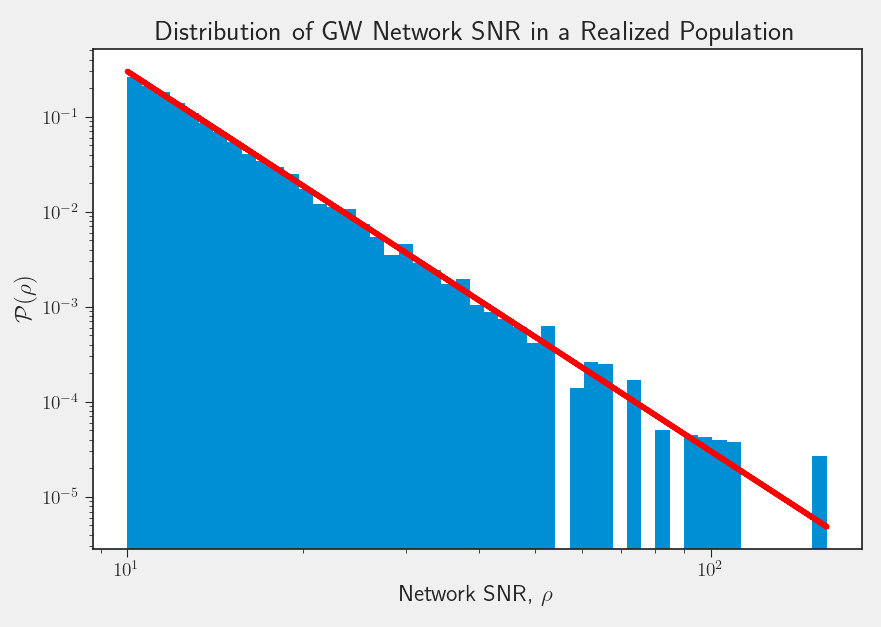
\includegraphics[width=0.8\linewidth]{rho_dist}
            \caption[Distribution of GW network SNR]{
                Distribution of GW network SNR, from a particular realisation of a
                population (specifically one with standard assumpations about binary
                parameters, except that the spin distribution is uniform). The red line
                is the curve given by theoretical considerations, which for a threshold
                SNR of 10, corresponds to $f(\rho) = 3\rho_{th}^3 / \rho^4 = 3000 /
                \rho^4$.
            }
            \label{fig:rho_dist}
        \end{figure}


        Furthermore, for these samples, the GW network SNR is higher in value if:

        \begin{itemize}

            \item The `event' is closer by, i.e. $D_L$ is low.

            \item The binary merges with the orbital plane face on, i.e. $\iota$ is low

            \item Both $D_L$ and $\iota$ are low, although this is a small part of the
                $D_L-\iota$ parameter space, and hence is less probable.

        \end{itemize}

        This implies a connection between the two parameters, and indeed this $D_L-\iota
        $ connection is well studied in the literature (see \cite{schutz_2011} \&
        \cite{seto_2015} for discussions on the same). This relation was also verified
        to hold within the population generated, which is shown in figure
        \ref{fig:dl_iota_correlation}. Note that some parts of the $D_L - \iota$
        parameter space are not at all populated by the samples, which reaffirms the
        fact that distant, edge-on mergers are disfavoured when such systems are being
        explored via GW.

        \begin{figure}[htpb]
            \centering
            \includegraphics[width=0.8\linewidth]{iota_dl_colorcoded}
            \caption[$D_L-\iota$ correlation in the population]{
                Plot of the luminosity distance v/s the inclination angle for events in
                the population, color coded by the SNR. Note that only events whose SNR
                > 10 (the SNR threshold) are considered here.  This shows that the
                generated population also exhibits the relation as expected from theory.
            }
            \label{fig:dl_iota_correlation}
        \end{figure}

    \subsection{EM Checks}\label{sub:em_checks}

    The only EM component which has to be validated is the code which imposes the jet
    structure (Eq. \ref{eq:dE_dOmega}-\ref{eq:eiso}), once the energetics of the jet are
    computed via Eq. \ref{eq:e_kin_jet}-\ref{eq:Omega_h}.\\
    In order do this, one extracts the $\theta_v$ samples from the generated population,
    which can be done using the relation $\theta_v = \min(\iota, \pi - \iota)$. Then, a
    common baseline is achieved by setting the value of $E_{kin, jet} = 10^{49} \text{
    erg}$ for all samples, regardless of the actual value if the binary parameters were
    to be taken into consideration. This is necessary to remove the variation of the
    structure with the intrinsic jet energetics, which is intimately related to the
    binary parameters.\\
    Then with this constraint applied, the value of $E_{iso}(\theta_v)$ is computed
    using Eq.  \ref{eq:dE_dOmega}-\ref{eq:eiso}. It is seen from Fig.
    \ref{fig:jet_struct} that jet structure is being imposed correctly and according to
    what is expected from theory.

    \begin{figure}[H]
        \centering
        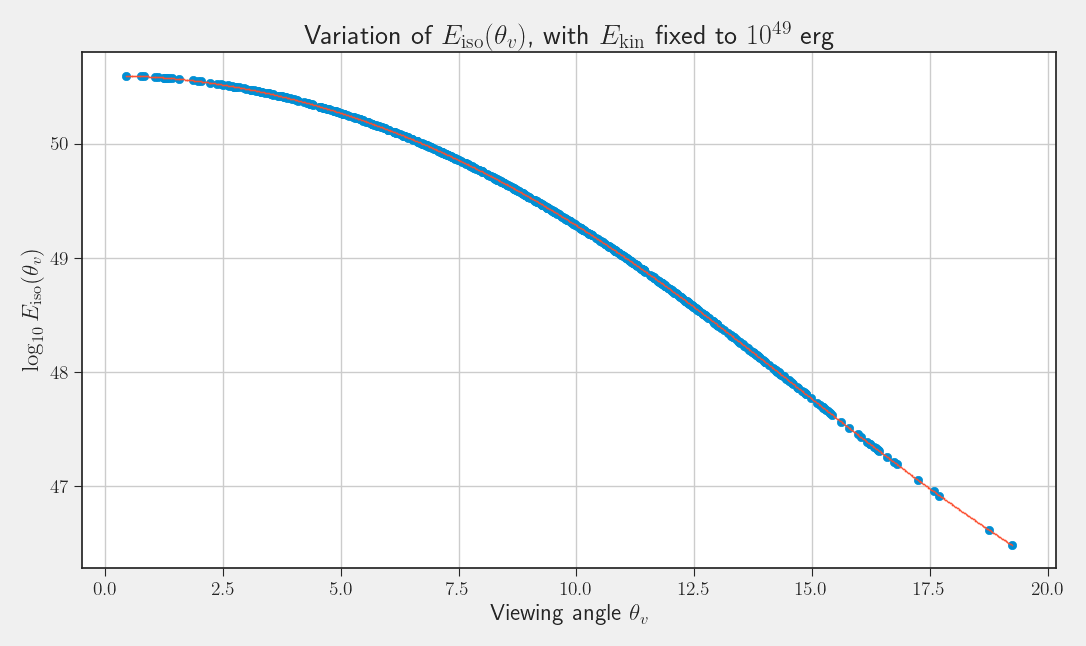
\includegraphics[width=0.8\linewidth]{jet_struct}
        \caption[Validation of the jet structure code]{
            Validation of the jet structure code, using the process mentioned in text.
            The blue scatter points are the values computed for $E_{iso}(\theta_v)$ for
            parameters from a population with $E_{kin, jet}$ set to $10^{49}$ erg,
            whereas the red line is that computed from theory for a jet with the same
            kinetic energy.
        }
        \label{fig:jet_struct}
    \end{figure}

    One additional check was performed to confirm the distribution of simulated binary
    mergers which led to jets. The number of  mergers which launched a jet with a
    fluence greater than some particular value was plotted, as a function of the
    particular fluence value. In other words, if $\mathcal{N}(>\mathcal{F})$ is the
    number of simulated mergers with a fluence greater than $\mathcal{F}$, then the
    behaviour of $\mathcal{N}(> \mathcal{F})$ was investigated in the simulated
    population.\\
    If the jet structure and spatial distribution codes were working to mimic what is
    observed in reality, the resulting structure should be isotropic but inhomogenous,
    as the sources would be cosmological in nature but appear isotropically distributed
    in the local universe. As for the expected behaviour of $\mathcal{N}(>
    \mathcal{F})$, this would mean that for large values of $\mathcal{F}$ it would
    behave as $\mathcal{F}^{-1.5}$ but would significantly deviate from this behaviour
    for lower values of $\mathcal{F}$.

    \begin{figure}[H]
        \centering
        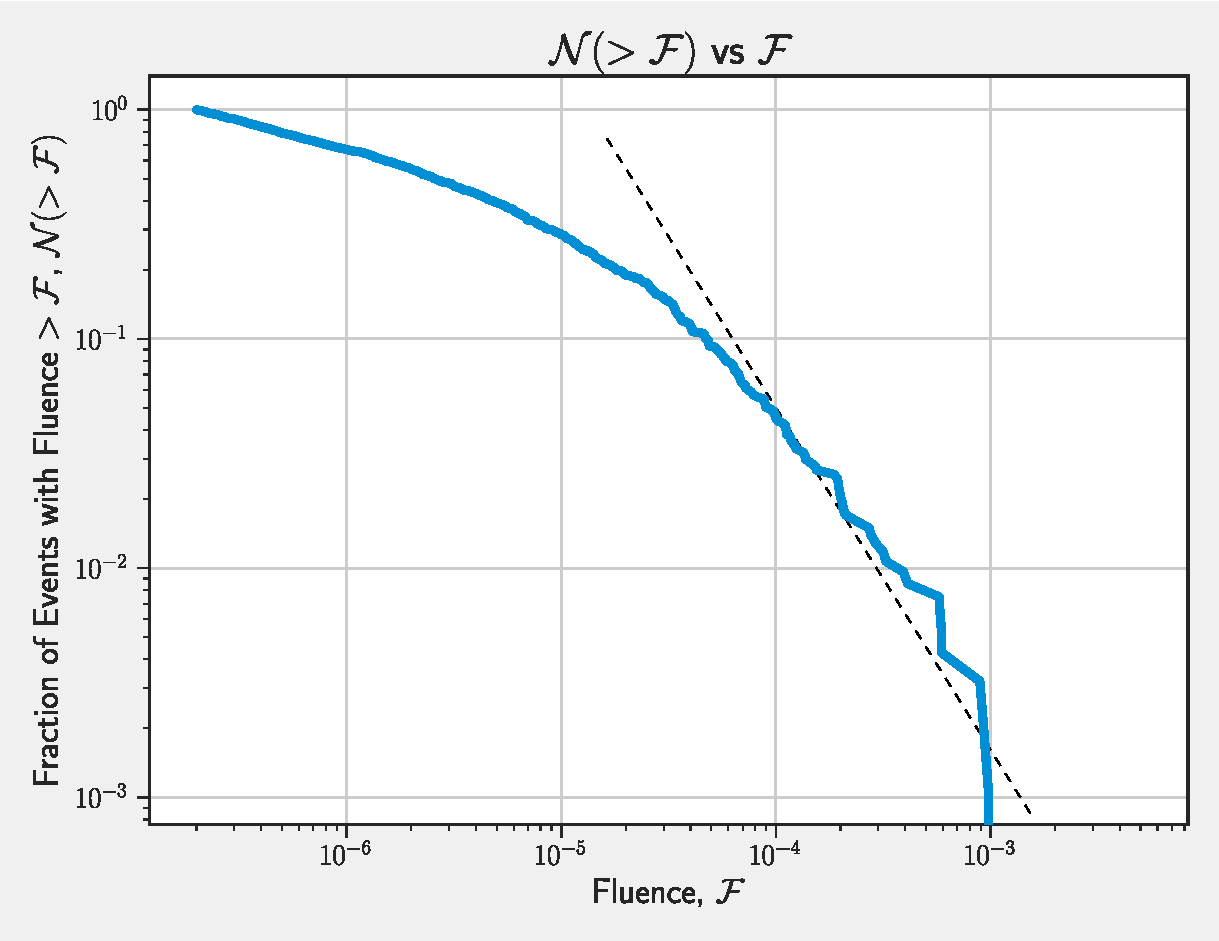
\includegraphics[width=0.9\linewidth]{number_fluence}
        \caption[Variation of $\mathcal{N}(> \mathcal{F})$ with $\mathcal{F}$]{
            Variation of $\mathcal{N}(> \mathcal{F})$ with the fluence $\mathcal{F}$.
            Note the significant deviation of this function from the $\sim
            \mathcal{F}^{-1.5}$ behaviour at lower values of the fluence.
        }
        \label{fig:number_fluence}
    \end{figure}

    From Fig.\ref{fig:number_fluence}, it is seen that the distribution of simulated
    mergers which launch a jet mimics the observed distribution of SGRBs in the
    Universe, and so the jet structure and source distribution codes are satisfactory.

    As an additional check for the jet structure imposition, a few prototypical binary
    mergers are considered, where each prototype is identified by the mass ratio,
    $\mathcal{Q}$, varied as $\mathcal{Q} = \frac{3}{1.4}, \frac{5}{1.4},
    \frac{10}{1.4}$. The variation of the fluence with the black hole spin, $\chi_{BH}$
    and the viewing angle, $\theta_v$ is what is studied in each prototypical case.
    These are given in Figs.\ref{fig:fluence_thetav+spin(3)} --
    \ref{fig:fluence_thetav+spin(5)}.

    \begin{figure}[H]
        \centering
        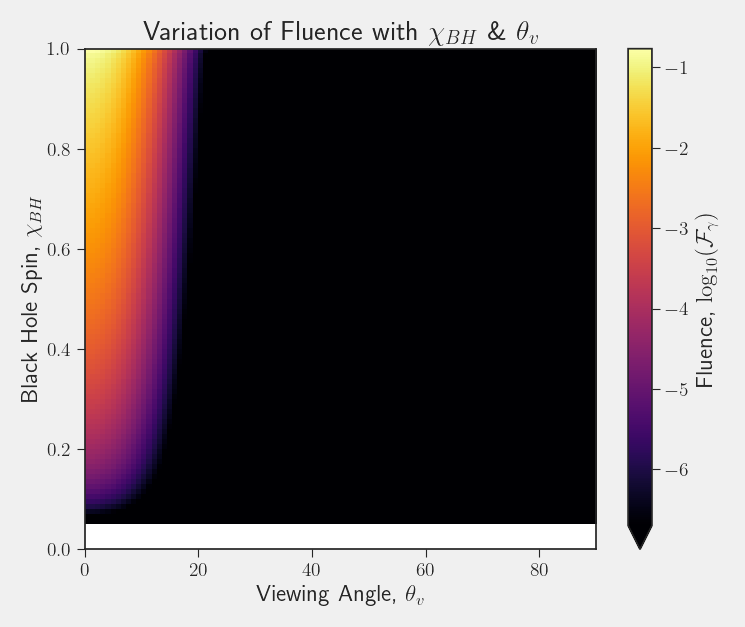
\includegraphics[width=0.8\linewidth]{fluence_thetav+spin(3)}
        \caption[Variation of $\mathcal{F}(\chi_{BH}, \theta_{v})$ for a
        $\mathcal{Q}=3:1.4$ NSBH binary merger]{
            The variation of fluence with the viewing angle and the black hole spin for
            a binary merger with a mass ratio of $\mathcal{Q}=3:1.4$. Here the regions
            of the $\chi_{BH}-\theta_v$ parameter space in white are those regions where
            no disc is produced, and hence the outgoing fluence is 0.
        }
        \label{fig:fluence_thetav+spin(3)}
    \end{figure}

    As can be seen from these figures:

    \begin{itemize}

        \item The higher the mass ratio of the merging NSBH system, the lower the
            probability for a jet to be launched. This is because the inspiralling NS
            plunges into the BH more often than not, thus undergoing little to no tidal
            disruption. Thus, the possibility of disc formation, and thus jet launching
            is very low in very asymmetric binaries.

        \item With asymmetric binary mergers, only if the black hole spin is high enough
            will there be any possibility of jet launching. This is because with a high
            enough black hole spin, the inspiralling NS can become tidally disrupted,
            and thus a massive disc can be formed using which a jet can be launched.
            However, it is highly unlikely that such high black hole spins are actually
            physical.

    \end{itemize}

    \begin{figure}[H]
        \centering
        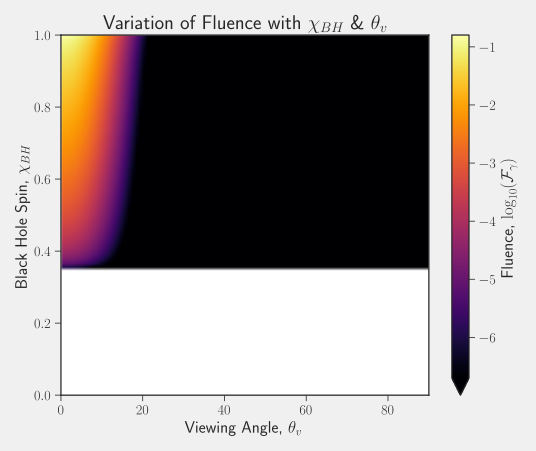
\includegraphics[width=0.8\linewidth]{fluence_thetav+spin(5)}
        \caption[Variation of $\mathcal{F}(\chi_{BH}, \theta_{v})$ for a
        $\mathcal{Q}=5:1.4$ NSBH binary merger]{
            The variation of fluence with the viewing angle and the black hole spin for
            a binary merger with a mass ratio of $\mathcal{Q}=5:1.4$. Note that in this
            case the region where a disc is not produced is a much larger fraction of
            the parameter space, compared to Fig.\ref{fig:fluence_thetav+spin(3)}.
        }
        \label{fig:fluence_thetav+spin(5)}
    \end{figure}

    Thus, from Figs.\ref{fig:fluence_thetav+spin(3)} --
    \ref{fig:fluence_thetav+spin(5)}, it can be seen that symmetric binary mergers will
    produce much brighter jets for a given black hole spin, and these jets will be seen
    out to higher viewing angles. This fact will be useful while discussing the analysis
    of the various populations synthesized, their EM/GW/joint detectabilities.
    Furthermore, from these figures, it is also verified that the code which imposes the
    jet structure and energetics is working correctly, since these conclusions about the
    EM detectabilities of NSBH binary mergers are the ones reached in literature as
    well (see \ref{sec:nsbh} for a brief overview of the literature discussing
    these results)

    \begin{figure}[ht]
        \centering
        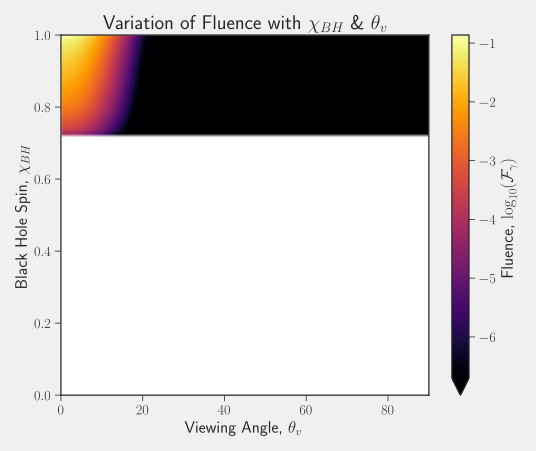
\includegraphics[width=0.8\linewidth]{fluence_thetav+spin(10)}
        \caption[Variation of $\mathcal{F}(\chi_{BH}, \theta_{v})$ for a
        $\mathcal{Q}=10:1.4$ NSBH binary merger]{
            The variation of fluence with the viewing angle and the black hole spin for
            a binary merger with a mass ratio of $\mathcal{Q}=10:1.4$. Here the region
            of parameter space where the jet is launched is extremely restricted, as the
            NSBH binary in question is very asymmetric in its masses.
        }
        \label{fig:fluence_thetav+spin(10)}
    \end{figure}

\section{Summary}

    In this chapter, the various populations that will be used to probe the EM
    counterparts of NSBH mergers were briefly explained. Along with this exposition, a
    summary of the various tests carried out was given, wherein the tests made sure that
    the internal code that computes the GW SNR, calculates jet energetics (from formulae
    derived as fits to numerical relativity simulations), imposes jet structures etc.,
    gave preliminary results which align with the theoretical results.\\
    In the coming chapters, the framework set up in this and the previous chapters for
    the synthesis and analysis of the populations and NSBH merger events will be used to
    derive results about the properties of NSBH binary mergers and their subsequent EM
    prompt counterparts.
  % About Popln Syn. Code
                      % TODO: add more info

    \chapter{Population Analysis}\label{chp:analysis}

\section{Summary}
  % Science from Population
                      % TODO

    \chapter{NS Merger Candidates in GWTC-2}\label{ch:candidates}

\section{About GWTC-2}

    The first half of the third observing run (O3a) of the LVC started on the 1st of
    April 2019, and went on till 30th of September, 2019.  Following this, instrumental
    upgrades were made during the month of October and the second half of the third
    observing run (O3b) was started on the 1st of November. Due to the global pandemic,
    the observing run had to be prematurely suspended on 30th of March, 2020.\\
    Starting with O3, alerts were distributed via the public alerts section of
    Gravitational-wave Candidate Event Database (GRACE-DB). If triggers were registered
    that passed the detection threshold of the LVC network during observational runs,
    online parameter estimation was done using the raw GW data, and low latency
    estimates of the rough sky position, component masses and luminosity distance was
    made available for observers in the EM regime. This allowed for rapid follow-up in
    various bands of the electromagnetic spectrum, and these observations were reported
    and cross-verified using NASA's GRB Coordinates Network (GCN). Using the circulars
    reported in the GCN for NSBH/BNS events of interest, along with the low-latency
    information from GRACE-DB, O3a's non-BBH candidate events have been collected in
    table \ref{tab:gcns}.\\
    More detailed analysis of these events in the months following has led to at least
    53 events in the third observing run alone. These can be classified as:
    \begin{itemize}

        \item 37 Binary Black Hole (BBH) merger candidates.

        \item 7 BNS merger candidates. Of these, only 1 corresponds to O3a, which is the
            event GW190425 discussed in the chapter \ref{sec:190425}.

        \item 4 events in the mass gap, which are events with compact objects with
            masses of 3-5 $M_{\odot}$.

        \item 5 NSBH merger candidates. Of these, only 1 has been confirmed officially,
            which is the event GW190814.

    \end{itemize}

    Of these, 26 events were officially confirmed and 13 new events were reported for
    the first time in \cite{abbott_2020A}, and it is from there that the posterior
    distributions of the various parameters (such as inclination angle $\iota$,
    luminosity distance $D_L$ etc) are used for further analysis.  Note also that there
    are several marginal events that have been reported, in that they have
    non-negligible probability distributed between two classifications. For example, the
    event GW190426\_152155 has significant probability split between it being a
    terrestrial event (58 \%) and a NSBH/BNS/Mass Gap event (cumulatively 42\%). Without
    a significant EM counterpart, this event cannot be confidently placed in either of
    the classes, and thus warrants further analysis. This is the subject of chapter
    \ref{sec:190426}.

    \begin{table}[H]  % now this is how you format a table ;)
        \centering
        \setlength{\extrarowheight}{0pt}
        \addtolength{\extrarowheight}{\aboverulesep}
        \addtolength{\extrarowheight}{\belowrulesep}
        \setlength{\aboverulesep}{0pt}
        \setlength{\belowrulesep}{0pt}
        \begin{tabular}{cccccc}
            \toprule
            \rowcolor[rgb]{0.71,0.851,1}
            \begin{tabular}[c]{@{}>{\cellcolor[rgb]{0.71,0.851,1}}c@{}}
                \textbf{GRACE-DB} \\
                \textbf{Superevent} \\
                \textbf{ID}
            \end{tabular} &
            \textbf{$\mathcal{P}$(BBH)} & \textbf{$\mathcal{P}$(BNS)} &
            \textbf{$\mathcal{P}$(MassGap)} & \textbf{$\mathcal{P}$(NSBH)} &
            \textbf{$\mathcal{P}$(Terr)}  \\
            \hline \uline{S190426c} & 0 & 24 & 12 & 6 & 58\\
            S190910h & 0 & 61 & 0 & 0 & 39 \\
            S200213t & 0 & 63 & 0 & 0 & 37 \\
            S191213g & 0 & 77 & 0 & 0 & 23 \\
            S190901ap & 0 & 86 & 0 & 0 & 14 \\
            \uline{S190425z} & 0 & \textbf{\textgreater{}99} & 0 & 0 & 0 \\
            S190930s & 0 & 0 & 95 & 0 & 5 \\
            S190923y & 0 & 0 & 0 & 68 & 32 \\
            S190930t & 0 & 0 & 0 & 74 & 26 \\
            S191205ah & 0 & 0 & 0 & 93 & 7 \\
            S190910d & 0 & 0 & 0 & 98 & 2 \\
            S190814bv & 0 & 0 & 0 & \textbf{\textgreater{}99} & 0 \\
            \bottomrule
        \end{tabular}
        \caption[Candidate Merger Events and GRACE-DB Superevent IDs]{
                List of candidate merger events and the probability of
                classification (reported in \%) for each non-BBH event reported
                during O3a. Here the GRACE-DB superevent ID is used (instead of the
                GWTC-2 event ID), since for a particular GW event, the superevent
                collects both the EM followup as well as GW trigger information
                within GRACE-DB. The probabilities are assigned using the process
                described in \cite{kapadia_2020}, and are reported
                in GRACE-DB. The events underlined are discussed in more detail in
                later chapters.
            }
    \end{table}


    \begin{table}[H]
        \centering
        \setlength{\extrarowheight}{0pt}
        \addtolength{\extrarowheight}{\aboverulesep}
        \addtolength{\extrarowheight}{\belowrulesep}
        \setlength{\aboverulesep}{0pt}
        \setlength{\belowrulesep}{0pt}
        \begin{tabular}{cccc}
            \toprule
            \rowcolor[rgb]{0.71,0.851,1}
            \textbf{UID} & \textbf{FAR} & \textbf{$D_L$ (Mpc)} &
            \begin{tabular}[c]{@{}>{\cellcolor[rgb]{0.71,0.851,1}}c@{}}
                \textbf{Error in $D_L$} \\
                \textbf{(Mpc)}
            \end{tabular}  \\
            \hline
            \uline{S190426c} & 1 per 1.6276 yr & 377 & 100 \\
            S190910h & 1.1312 per yr & 230 & 88 \\
            S200213t & 1 per 1.7934 yr & 201 & 80 \\
            S191213g & 1.1197 per yr & 201 & 81 \\
            S190901ap & 1 per 4.5093 yr & 241 & 79 \\
            \uline{S190425z} & 1 per 69834 yr & 158 & 43 \\
            S190930s & 1 per 10.534 yr & 709 & 191 \\
            S190923y & 1.5094 per yr & 438 & 133 \\
            S190930t & 1 per 2.0536 yr & 108 & 38 \\
            S191205ah & 1 per 2.5383 years & 385 & 164 \\
            S190910d & 1 per 8.5248 years & 606 & 197 \\
            S190814bv & 1 per 1.559e+25 years & 241 & 26 \\
            \bottomrule
        \end{tabular}
        \caption[Candidate Merger Events and FARs]{
                List of candidate merger events and the probability of
                classification for each non-BBH event reported during O3a. FAR
                refers to the False Alarm Rate (in number of events per year or
                equivalently in Hz$^{-1}$), and $D_L$ is the luminosity distance.
                Both these values are those reported in GRACE-DB corresponding to
                each event. The events underlined are discussed in more detail in
                later chapters.
            }
    \end{table}

    \begin{table}[H]
        \centering
        \setlength{\extrarowheight}{0pt}
        \addtolength{\extrarowheight}{\aboverulesep}
        \addtolength{\extrarowheight}{\belowrulesep}
        \setlength{\aboverulesep}{0pt}
        \setlength{\belowrulesep}{0pt}
        \begin{tabular}{ccccc}
            \toprule
            \rowcolor[rgb]{0.71,0.851,1}
            \textbf{UID} &
            \textbf{FERMI-LAT} &
            \textbf{FERMI-GBM} &
            \textbf{SWIFT/BAT} &
            \textbf{INTEGRAL} \\
            \hline
            \uline{S190426c} & 24342 & 24248 & 24255 & 24242\\
            S190910h & 25742 & 25714 & 25718 & 25709 \\
            S200213t &
                27062 &
                {\cellcolor[rgb]{1,0.749,0.749}} \textcolor{red}{27056} &
                {\cellcolor[rgb]{1,0.749,0.749}} \textcolor{red}{27058} &
                27050 \\
            S191213g & 26412 & 26409 & 26410 & 26401 \\
            S190901ap & 25625 & 25610 & 25617 & 25605 \\
            \uline{S190425z} &
                24266 &
                24185 &
                24184, 24296 &
                \begin{tabular}{c}
                    24169, 24170 \\
                    24178, 24181
                \end{tabular} \\
            S190930s & 25895 & 25886 & 25889 & 25872 \\
            S190923y & 25834 & 25823 & 25846 & 25815, 25825 \\
            S190930t & 25898 & 25887 & 25888 & 25880 \\
            S191205ah & 26363 & 26359 & 26365 & 26531 \\
            S190910d & 25717 & 25699 & 25704 & 25698 \\
            S190814bv & 25385 & 25326 & 25341 & 25323 \\
            \bottomrule
        \end{tabular}
        \caption[Candidate merger events and relevant GCNs]
            {
                List of candidate merger events and the probability of
                classification for each non-BBH event reported during O3a. Here the
                GCN Circular number reporting the findings of the particular
                instrument in the column heading is reported, corresponding to each
                event. The events underlined are discussed in more detail in later
                chapters. GCNs marked with red should be ignored during analysis
                since they correspond to times when the respective instruments were
                in the South Atlantic Anomaly (SAA).
            }
        \label{tab:gcns}
    \end{table}

\section{Analysis of GW190425}\label{sec:190425}

    GW190425 (or S190425z in GRACE-DB) is a GW trigger which was recorded by the LVC on
    25th April, 2019 at 08:18 UTC. At the time of this trigger, the Hanford site of LIGO
    (H1) was undergoing maintenance, whereas the Livingston site (L1) of LIGO and the
    VIRGO detector were both operational. However, at the VIRGO detector this event was
    sub-threshold, effectively making this event a single-detector trigger. As a
    consequence, the LVC sky localisation area was wider than as compared to GW170817,
    and EM follow-up was constrained to serendipitious observations by satellites which
    happened to be observing the same area of the sky, or to diminished coverage by
    satellites due to observational schedules.

    Initial work was carried out to reproduce the results of \cite{saleem_2020B}, where
    the authors use a frequentist approach to discuss the possibility of a relativistic
    jet from the binary neutron star (BNS) merger event GW190425\footnote{
        At the time of the writing of the paper, this event was still not confirmed as a
        bona-fide GW event, and so it was denoted by GRACE-DB as S190425z. Consequently,
        several key pieces of information (such as the luminosity distance and
        inclination angle posteriors) from the GW inference was not yet public, and had
        to be worked around. See text for more details.
    }. In \cite{saleem_2020B}, three key ideas  are developed which are described in
    detail in the following sections.

    \subsection{Constraints on the \texorpdfstring{$D_L-\iota$}{dL-iota} Posterior}
    \label{sec:dl-iota_posterior}

    At the time of writing of \cite{saleem_2020B}, only the low-latency information was
    made public. Consequently, information about the inclination angle of this event was
    not released. However, both the luminosity distance ($D_L$) and inclination angle
    ($\iota$) of the event are required for the electromagnetic analysis of the
    event\footnote{
        The former is used to calculate the fluence, and the latter is directly related
        to the viewing angle, which in turn decides the observed isotropic equivalent
        energy (see Eq. \ref{eq:6})
    }. To solve this issue, a known correlation between the luminosity distance $D_L$
    and $\iota$ (see \cite{schutz_2011}, \cite{seto_2015}) was used to infer the
    distribution of $\iota$ for this event, which was possible since the former was
    publicly known.\\
    The following are the other publicly released information relevant to the problem,
    and can be used to constrain the $D_L-\iota$ joint distribution:
    \begin{itemize}

        \item The posterior probability of the event being a BNS merger is $>$ 99 \%,

        \item The event was observed by the LIGO Livingston (L1), and Virgo (V1)
            detectors, whereas the LIGO Hanford (H1) detector was not observing.
            However, at V1 the signal-to-noise ratio (SNR) was below the threshold and
            thus this event was a single detector trigger.

        \item The preliminary luminosity distance estimate is given by $D_L$ = 155 $\pm$
            41 Mpc.

    \end{itemize}

    Using these inputs the $D_L-\iota$ space is constrained as follows.
    \begin{enumerate}

        \item A population of BNS mergers is simulated, such that they are uniformly
            distributed in the comoving volume, with the inclination angle of the
            binaries being such that $\cos \iota \in [-1, 1]$. This also means that the
            luminosity distance is initially distributed such that $\mathcal{P}(D)
            \propto D^2$ upto some threshold distance. For the purposes of the
            simulations, this threshold distance is set to be the distance corresponding
            to the 99\% percentile of a Gaussian with a mean of 155 Mpc and a standard
            deviation of 41 Mpc. In practice, it is the maximum distance up till which
            the comoving and the luminosity distances can be used interchangeably, which
            corresponds to a redshift of roughly 0.1.

        \item The NS masses are uniformly distributed between 1-2 $M_{\odot}$. This
            enforces the constraint that from the analysis of the GW waveform, the event
            has > 99 \% probability of being a BNS merger.

        \item Then, the optimal SNR is computed for each realisation using the
            restricted post-Newtonian (PN) waveform (RWF) (see \cite{cutler_1994},
            \cite{kastha_2020}). Usually, the process of matched filtering is
            done to detect GW signals amongst background noise, where various template
            waveforms are cross-correlated with the observed data. These templates all
            correspond to mergers with various signal parameters such as masses, spins
            etc., and the template which maximizes the SNR is the optimal template, with
            the corresponding SNR being the optimal SNR, defined as :
            \begin{equation}
                \rho = \sqrt{4 \int_0^\infty \dfrac{|\tilde{h}(f)|^2}{S_h(f)} df}
            \end{equation}
            where $S_h(f)$ is the detector's power spectral density (PSD) and
            $\tilde{h}(f)$ is the frequency domain gravitational waveform.  For the RWF,
            this is given as $\tilde{h}(f) = \mathcal{A} f^{-7/6} e^{i \psi(f)}$, where
            $\mathcal{A}$ is the amplitude and $\psi(f)$ is the frequency domain GW
            phase.  In this scheme, the PN corrections to the amplitude of the waveform
            are ignored but the phase is accurately accounted for, since GW parameter
            estimations are most sensitive to the phase of the waveform
            (\cite{poisson_1995}). Using the RWF, the optimal SNR for compact binary
            coalescences can be written as :
            \begin{equation}
                \rho(m_1, m_2, D_L, \theta, \phi, \psi, \iota) =
                    \sqrt{
                        4 \dfrac{\mathcal{A}^2}{D_L^2}
                        \left[
                                 F_{+}^2(\theta, \phi, \psi)(1 + \cos^2\iota)^2 +
                                 4F_{\times}^2(\theta, \phi, \psi)\cos^2\iota
                        \right]
                        I(M)
                    }
            \end{equation}
            where $F_{+, \times}(\theta, \phi, \psi)$ are the antenna pattern functions
            for the 'plus' and 'cross' polarisations, $\mathcal{A} = \sqrt{5/96}
            \pi^{-2/3} \mathcal{M}^{5/6}$. Here, $\mathcal{M}$ is the chirp mass, which
            is related to the total mass M by $\mathcal{M} = M \eta^{3/5}$, where $\eta
            = \frac{m_1 m_2}{M^2}$ is the symmetric mass ratio of the system and $m_1,
            m_2$ are the component masses. The four angles $(\theta, \phi, \psi, \iota)$
            describe the location and orientation of the source with respect to the
            detector. $I(M)$ is the frequency integral defined as :
            \begin{equation}
                I(M) =
                    \int_0^\infty \dfrac{f^{-7/3}}{S_h(f)} df \approx
                    \int_{f_{low}}^{f_{LSO}} \dfrac{f^{-7/3}}{S_h(f)}
            \end{equation}
            where, $f_{low}$ is the lower seismic cut-off for the detectors and $f_{LSO}
            = \dfrac{1}{6^{3/2}\pi M}$, which is the GW frequency at the last stable
            orbit for a BBH merger with total mass M.  To compute the optimal SNR in L1
            and V1, the best reported O2 sensitivities were used as conservative O3
            sensitivities, as an input for $S_h(f)$.  As the trigger is an L1
            single-detector trigger, the conditions that SNR < 4 at V1 and the network
            SNR > 9 are enforced. The former is motivated by the single-detector
            threshold of the GstLAL pipeline, whereas the latter is motivated by the
            fact that the network SNR of all O1/O2 events were > 9.

        \item From the resulting population, a sub-population is extracted such that the
            luminosity distance follows a Gaussian distribution with a mean of 155 Mpc
            and a standard deviation of 41 Mpc. This is done so as to impose the
            constraint applied by the luminosity distance posterior distribution
            released by the LVC.

    \end{enumerate}

        The resulting 2D distribution of $D_L-\iota$ of this sub-population is shown in
        the figure below. This is used further on, as the prior for studying the
        possibility of a sGRB from GW190425.

    \begin{figure}[H]
        \centering
        \def\svgwidth{0.9\textwidth}
        \input{figures/saleem+Fig1.pdf_tex}
        \caption[$D_L-\iota$ Posterior distribution.]{
                    Constraints on the $D_L-\iota$ joint distribution, obtained from
                    imposing the observed properties of S190425z/GW190425.
        }
        \label{fig:dl_iota}
    \end{figure}

    \subsection{Calculation of the Apparent structure}

    Assuming the intrinsic jet structure models described before (in Sec.
    \ref{sec:bns}), the apparent isotropic equivalent energy is calculated using the
    equation (as in \cite{salafia_2015} and
    \cite{biscoveanu_2020}):

     \begin{equation}
         \label{eq:6}
         E_{iso}(\theta_v) =
             \dfrac{1}{2\pi}
             \int_{0}^{2\pi} d\phi \int_{0}^{\theta_{max}} d\theta
             \sin \theta
             \dfrac{\epsilon(\theta)}{\Gamma(\theta)^4
             [1 - \beta(\theta) \cos \alpha_v]^3}
     \end{equation}

    where:
    \begin{itemize}

        \item $\theta_v$ is the viewing angle of the observer.

        \item $\epsilon(\theta)$ is the normalised energy profile function.

        \item $\alpha_v$ is the angle between the line of sight and the direction to the
            jet element at $(\theta, \phi)$, given by $\cos \alpha_v = \cos \theta_v
            \cos \theta + \sin \theta_v \sin \theta \cos \phi$.

        \item $\theta_{max}$ is the upper cut-off of polar integration\footnote{
                Such a cutoff can occur because the edge of the jet has been reached, or
                that the gamma-ray emission efficiency is lowered below a threshold, and
                so emission is negligible beyond $\theta_{max}$.
            }.

    \end{itemize}

    Thus, depending on the underlying intrinsic structure assumed (be it Gaussian or
    tophat jet), using Eq. \ref{eq:6} one can infer the apparent structure of the jet.
    Note that this is the variation of the (apparent) isotropic equivalent energy
    ($E_{iso}$) at various viewing angles ($\theta_v$), and hence gives how the sGRB
    jet, if launched, would appear to an observer at an angle to the jet's axis. This
    variation is shown in Fig. \ref{fig:e_iso}, and is used a prior for further
    analysis.

    \begin{figure}
        \centering
        \def\svgwidth{\textwidth}
        \input{figures/e_iso.pdf_tex}
        \caption[Variation of the apparent isotropic equivalent energy,
                 for observers at different viewing angles]{
                 Variation of the apparent isotropic equivalent energy, for observers at
                 different viewing angles. The figure shows both the top-hat (dark red)
                 and Gaussian (dark green) jet structures, with $E_{tot., \gamma} =
                 10^{49}$ ergs. $\theta_j$ for the top-hat jet and $\theta_c$ for the
                 Gaussian jet are both $5^{\circ}$ (marked with vertical solid bright
                 red line), and $\Gamma_0$ in both cases is 100. The horizontal dashed
                 black line denotes $E_{iso}(0)$. The orange, dash-dotted line and the
                 blue dotted lines are the tophat and Gaussian intrinsic jet structures,
                 represented as $4\pi\epsilon(\theta_v)$. For the solid green curve, the
                 entire jet emits gamma-rays, whereas for the dashed and dashed-dotted
                 green curves the emission is restricted to regions where $\Gamma \beta
                 > 15$ and $\Gamma \beta  > 30$, leading to limits in the polar
                 integration of 9.74$^\circ$ (vertical dashed violet line) and
                 7.76$^\circ$ (vertical dash-dotted violet line) respectively.
        }
        \label{fig:e_iso}
    \end{figure}

    \subsection{Monte-Carlo simulations}
    \label{sec:mc_sim}

    Using the information from the previous analyses and further priors motivated from
    them, a Monte-Carlo simulation was run where $10^5$ realisations of the Gaussian jet
    were made. Their model fluence was compared with what was reported by INTErnational
    Gamma-Ray Astrophysics Laboratory (INTEGRAL).\\ Around the time of the GW trigger,
    INTEGRAL was observing the entire AdvLIGO/VIRGO localisation region and according to
    \cite{minaev_gcn_2019}, saw a low SNR short duration ($\sim$ 1s) excess roughly 6s
    after the merger. Further analysis reported a fluence of $(1.6 \pm 0.4) \times
    10^{-7} \text{ erg/cm}^2$. The priors used for the various parameters of the
    Gaussian jets realised are as given in table \ref{table:priors}.

    \begin{table}[H]
        \centering
        \setlength{\extrarowheight}{0pt}
        \addtolength{\extrarowheight}{\aboverulesep}
        \addtolength{\extrarowheight}{\belowrulesep}
        \setlength{\aboverulesep}{0pt}
        \setlength{\belowrulesep}{0pt}
        \begin{tabular}{|c|c|c|c|}
            \toprule
            & $E_{tot., \gamma}$ (erg) & $\Gamma_0$ & $\theta_c$ \\
            \hline
            \rowcolor[rgb]{0.812,0.812,0.812}
            \textbf{Uniform Energy Prior} & $ 44 < \log_{10}(E_{tot., \gamma}) < 51$ &
            $5 < \Gamma_0 < 500$ & $3^{\circ} < \theta_c < 20^{\circ}$ \\
            \hline
            \begin{tabular}[c]{@{}c@{}}
                \textbf{Broken Power Law} \\
                \textbf{Energy Prior}
            \end{tabular} &
            \begin{tabular}[c]{@{}c@{}}
                BPL \{ [$5 \times 10^{47}, 10^{50}; -0.53$], \\{[}$10^{50}, 5 \times 10^{51}; -3.5$] \}
            \end{tabular} &
            $ 100 \Gamma_0 500$ & $3^{\circ} < \theta_c < 20^{\circ}$  \\
            \bottomrule
        \end{tabular}
        \caption[Priors on $E_{tot., \gamma}$, $\Gamma_0$ and $\theta_c$]{
            Priors on the total energy emitted in gamma-rays ($E_{tot., \gamma}$), bulk
            on-axis Lorentz factor ($\Gamma_0$) and core-angle ($\theta_c$). The
            notation used for the broken power-law distribution is explained below.
        }
        \label{table:priors}
    \end{table}

    Here, BPL$\{[5 \times 10^{47}, 10^{50}; -0.53], [10^{50}, 5 \times 10^{51}; -3.5]\}$
    is equivalent to:
    \begin{equation}
        \label{eq:7}
         P(E_{tot., \gamma}) \propto
        \begin{cases}
            E_{tot., \gamma}^{-0.53}, &
                5 \times 10^{47} \text{ ergs } <
                E_{tot., \gamma} <
                10^{50} \text{ ergs }  \\
            E_{tot., \gamma}^{-3.5}, &
                10^{50} \text{ ergs } <
                E_{tot., \gamma} <
                5 \times 10^{51} \text{ ergs }
        \end{cases}
    \end{equation}

    \begin{figure}[H]
        \centering
        \def\svgwidth{0.5\textwidth}
        \input{figures/bpl_demo.pdf_tex}
        \caption[Broken power law distribution from \cite{ghirlanda_2016}.]{
            The broken power law distribution as described in Eq. \ref{eq:7}.
        }
        \label{fig:bpl_demo}
    \end{figure}

    This particular distribution for the prior of $E_{tot., \gamma}$ is adopted since it
    is able to reproduce the fluence distribution observed, for values above the
    limiting fluence of $2 \times 10^{-7} \text{ erg/cm}^2$ (see \cite{mohan_2019}).
    Furthermore, the power-law indices are adopted from the luminosity function
    described in \cite{ghirlanda_2016}.

    In applying these priors, along with the $D_L-\iota$ prior and the fluence values of
    $2 \times 10^{-7}$ and $(1.6 \pm 0.4) \times 10^{-7}$ erg/cm$^2$ as upper limit and
    detections respectively, supplied by INTEGRAL, the marginalized posteriors for
    $\theta_c, \Gamma_0, \theta_v$ and $E_{tot., \gamma}$ are obtained. These are
    converted into $E_{iso}(0)$. The posterior distributions of the on-axis, apparent
    isotropic equivalent energy, for the two priors considered, is shown in Fig.
    \ref{fig:unif_bpl}. As is evident from seeing the figure, the INTEGRAL fluence is a
    good constraint for the priors. For the uniform prior case, considered as a
    detection, the posterior $E_{iso}(0)$ is tightly constrained to be between
    $3.51\times 10^{47} - 6.26 \times 10^{52}$ ergs, which shows that for an on-axis
    observer, the event would have appeared as a typical sGRB along with the GW event.
    Even considering as an upper-limit constrains $E_{iso}(0) \leq 1.48\times 10^{51}$,
    which is broadly in agreement with that observed for typical sGRBS.  On the other
    hand, the narrower, broken power-law prior is not constrained well with the INTEGRAL
    fluence. Considered as a detection, the 90\% credible posterior bounds on
    $E_{iso}(0)$ are $1.17\times10^{49}-1.3\times10^{51}$ ergs, whereas considered as an
    upper limit, $E_{iso}(0) \leq 7.69 \times 10^{50}$ erg. In both cases, the
    posteriors are sensitive to the choice of the prior, but nevertheless, one cannot
    rule out an sGRB jet which would have been seen by an on-axis observer.

    \begin{figure}[H]
        \begin{subfigure}{0.5\textwidth}
              \label{fig:unif}
              \centering
              \def\svgwidth{\textwidth}
              \input{figures/unif.pdf_tex}
        \end{subfigure}%
        \begin{subfigure}{0.5\textwidth}
              \label{fig:bpl}
              \centering
              \def\svgwidth{\textwidth}
              \input{figures/bpl_1.9.pdf_tex}
        \end{subfigure}
        \caption[Posterior distributions of the apparent on-axis isotropic equivalent
        energy $E_{iso}(0)$, for two assumed priors on the total energy emitted in
        gamma-rays, $E_{tot., \gamma}$]{
            Posterior distributions of the apparent on-axis isotropic equivalent energy
            $E_{iso}(0)$, for two assumed priors on the total energy emitted in
            gamma-rays, $E_{tot., \gamma}$. These figures give constraints on the
            $E_{iso}(0)$ of the sGRB associated with GW190425, assuming a Gaussian
            structured jet. \textbf{Left:} Grey histogram indicates the uniform priors
            on $\log_{10}(E_{tot., \gamma}/erg)$ in the range of [44 --- 51], and on
            $\theta_c$ in [3, 20] degrees.  \textbf{Right:} the same prior is used for
            $\theta_c$ but a broken power law prior is used for $E_{tot., \gamma}$. The
            orange histograms in both are a result of considering an INTEGRAL fluence
            upper limit of $2 \times 10^{-7} \text{ erg/cm}^2$, where the blue
            histograms in both are a result of considering an INTEGRAL fluence detection
            of $(1.6 \pm 0.4) \times 10^{-7} \text{ erg/cm}^2$. In both cases, the
            on-axis energy of a possible associated GRB is within the range of that of
            the cosmological sGRB population.
        }
        \label{fig:unif_bpl}
    \end{figure}

    %Write about the Monte-Carlo simulations undertaken to use the two pieces of
    %information from the two previous sections, to constrain the priors input, and see
    %whether the event S190425c could have possibly been a typical sGRB. Need to get
    %90\% credible intervals!

    \subsection{Using LIGO posteriors}

    In the time since the analysis in \cite{saleem_2020B} was carried out, the
    posteriors for the O3a events were released as part of the Gravitational Wave
    Transient Catalog (GWTC) 2 (see \cite{abbott_2020A}). These are now available as part
    of the event portal at the Gravitational Wave Open Science Center (GWOSC), which
    lists the files that store samples from posterior distributions for various
    parameters, for each event in GWTC-2. This allows one to use the actual posteriors
    for the inclination angle and the luminosity distance reported by the LVC. These are
    plotted in Fig. \ref{fig:dl-iota_post_updated}, below.\\

    \begin{figure}[H]
        \centering
        \def\svgwidth{\textwidth}
        \input{figures/dL-iota_updated.pdf_tex}
        \caption[$D_L-\iota$ posterior, with samples from the data released by LVC.]{
            Similar as \ref{fig:dl_iota}, but with samples for $D_L$ and $\iota$ from
            the posteriors released by the LVC, as part of the GWTC-2 data release.
        }
        \label{fig:dl-iota_post_updated}
    \end{figure}

    These posteriors for the parameters $\iota$ and $D_L$ will be more accurate than the
    ones generated in \S\S\ref{sec:dl-iota_posterior}, since those posteriors are
    generated by approximating the O3a detector noise curves using the conservative best
    estimate of O2. Hence using the actual detector noise around the time of the event
    and performing parameter estimation for the parameters of interest (which is done by
    LVC), and using the resultant posteriors will be more accurate for further
    analysis.\\
    Using these posteriors, the constraints on the energetics of a sGRB jet
    being powered by an event like GW190425 change slightly. This is shown in Fig.
    \ref{fig:unif_bpl_updated}.

    \begin{figure}[H]
        \begin{subfigure}{0.5\textwidth}
              \label{fig:unif_updated}
              \centering
              \def\svgwidth{\textwidth}
              \input{figures/unif_up.pdf_tex}
        \end{subfigure}%
        \begin{subfigure}{0.5\textwidth}
              \label{fig:bpl_updated}
              \centering
              \def\svgwidth{\textwidth}
              \input{figures/bpl_1.9_up.pdf_tex}
        \end{subfigure}
        \caption[Posterior distributions of the apparent on-axis isotropic equivalent
        energy $E_{iso}(0)$, with similar priors as Fig. \ref{fig:unif_bpl} but with LVC
        posterior samples as input.]{
            Posterior distributions of the apparent on-axis isotropic equivalent energy
            $E_{iso}(0)$, with similar priors as Fig.  \ref{fig:unif_bpl} but with LVC
            posterior samples as input.
        }
        \label{fig:unif_bpl_updated}
    \end{figure}

    Considering the INTEGRAL fluence as a detection, the posterior bounds on
    $E_{iso}(0)$ are $5.61 \times 10^{47} - 8.48 \times 10^{52}$ ergs. This again leads
    to the conclusion that for an on-axis observer, the sGRB jet would have been
    detectable. Considering the INTEGRAL fluence as an upper limit instead, givens that
    $E_{iso}(0) \leq 7.43 \times 10^{51}$ erg.  Similar to the previous case, the narrow
    broken-power law prior is not well constrained by the INTEGRAL fluence limits, which
    places the bounds $1.15 \times 10^{49}-1.11 \times 10^{51}$ ergs (considered as a
    detection) and $E_{iso}(0) \leq 6.74 \times 10^{50}$ erg (considered as an upper
    limit). In this case as well, the conclusion is the same, that the possibility of
    sGRB which would have been visible seen on-axis cannot be ruled out. However, this
    showcases the usefulness of the method described in \S \ref{sec:dl-iota_posterior},
    wherein the posterior for the parameter $\iota$ can be approximated and used for
    further analysis, without having to wait for this information to be released
    officially.

\section{Preliminary analysis of GW190426\_152155}\label{sec:190426}

    %Talk about the preliminary results of using the GW190426 posteriors, and how that
    %is not constraining enough. Also put comparison with the other "typical" GRBs.

    The event GW190426\_152155 is listed in GWTC-2 (\cite{abbott_2020A}) as an event with
    a network matched filter signal-to-noise ratio of 10.1, a false-alarm rate of 1
    event per 1.6276 yr and the component masses are $5.7^{+4.0}_{-2.3}$ $M_{\odot}$ and
    $1.5^{+0.8}_{-0.5}$ $M_{\odot}$. From GRACE-DB, this event has probabilities 0.58,
    0.24, 0.12, 0.06 respectively of being a Terrestrial, BNS merger, NSBH merger or
    MassGap merger event.\\ Although there were no significant excesses reported by any
    of the Gamma-ray satellites observing the LVC localisation area at the time of the
    GW trigger, the INTEGRAL satellite reported an upper limit fluence of $1.7 \times
    10^{-7} \text{ ergs/cm}^2$. With the priors as given in Table \ref{table:priors},
    this fluence upper limit reported by INTEGRAL is taken as the primary constraint.
    Similar to the process described in \S\ref{sec:mc_sim}, $10^5$ realisations of the
    jet are made, the apparent on-axis isotropic equivalent energy calculated, from
    which the fluence is computed and those realisations with a fluence beyond the upper
    limit are rejected. The resulting population has a distribution as given in Fig.
    \ref{fig:nsbh_unif_bpl}.\\
    As can be seen from Fig.\ref{fig:nsbh_unif_bpl}, at apparent on-axis isotropic
    equivalent energies below $10^{48}$ erg, the uniform prior differs appreciably from
    the posterior, whereas at higher energies the posterior and prior exhibit the same
    behaviour. In the case of the broken power-law prior, at all energies considered,
    the posterior and prior distributions are  the fluence upper limit offered by
    INTEGRAl doesn't offer tight constraints. This is because for both the priors, the
    posterior largely follows the same behaviour as the prior, thus indicating that the
    constraint applied is a poor one.

    \begin{figure}[H]
        \begin{subfigure}{0.5\textwidth}
              \label{fig:nsbh_unif}
              \centering
              \def\svgwidth{\textwidth}
              \input{figures/unif_nsbh.pdf_tex}
        \end{subfigure}%
        \begin{subfigure}{0.5\textwidth}
              \label{fig:nsbh_bpl}
              \centering
              \def\svgwidth{\textwidth}
              \input{figures/bpl_1.9_nsbh.pdf_tex}
        \end{subfigure}
        \caption[Posterior distributions of the apparent on-axis isotropic equivalent
        energy $E_{iso}(0)$, in the case of GW190426\_152155.]{
            Posterior distributions of the apparent on-axis isotropic equivalent energy
            $E_{iso}(0)$, for two assumed priors on the total energy emitted in
            gamma-rays, $E_{tot., \gamma}$. These figures give constraints on the
            $E_{iso}(0)$ of the sGRB associated with GW190426\_152155, assuming a
            Gaussian structured jet. \textbf{Left:} Grey histogram indicates the uniform
            priors on $\log_{10}(E_{tot., \gamma}/erg)$ in the range of [44 --- 51], and
            on $\theta_c$ in [3, 20] degrees. \textbf{Right:} the same prior is used for
            $\theta_c$ but a broken power law prior is used for $E_{tot., \gamma}$. The
            orange histograms in both are a result of considering an INTEGRAL fluence
            upper limit of $1.7 \times 10^{-7} \text{ erg/cm}^2$.
        }
        \label{fig:nsbh_unif_bpl}
    \end{figure}

    This process sees whether the models used for the analysis of GW190425 also apply to
    the NSBH event GW190426\_152155. Although the constraint is not very good in either
    case of the prior, the conclusion that there is the possibility of a sGRB jet which
    could have been detected had the observer been on-axis, cannot be ruled out
    completely. In this case, considering the constraint as an upper limit, the bounds
    are $E_{iso}(0) \leq 4.52 \times 10^{51}$ erg and $E_{iso}(0) \leq 6.81 \times
    10^{50}$ erg for the uniform prior and the broken power-law prior respectively.  As
    an additional check, table \ref{table:typical_grbs} lists the parameters for some of
    the typical, well-studied sGRBs. Comparing what was obtained after the analysis of
    GW190426\_152155 to the observed isotropic equivalent energy for these sGRBs, it can
    be seen that this NSBH event is still in the ballpark of cosmological sGRBs.

    \begin{table}
        \centering
        \setlength{\extrarowheight}{0pt}
        \addtolength{\extrarowheight}{\aboverulesep}
        \addtolength{\extrarowheight}{\belowrulesep}
        \setlength{\aboverulesep}{0pt}
        \setlength{\belowrulesep}{0pt}
        \begin{tabular}{ccccccc}
            \toprule
            \rowcolor[rgb]{1,0.741,0}
            \textbf{GRB ID} &
            \begin{tabular}[c]{@{}>{\cellcolor[rgb]{1,0.741,0}}c@{}}
                \textbf{Relevant} \\ \textbf{ GCN} \\ \textbf{ Notices}
            \end{tabular} &
            \begin{tabular}[c]{@{}>{\cellcolor[rgb]{1,0.741,0}}c@{}}
                \textbf{Duration} \\ \textbf{(ms)}
            \end{tabular} &
            \begin{tabular}[c]{@{}>{\cellcolor[rgb]{1,0.741,0}}c@{}}
                \textbf{Fluence} \\ \textbf{($\text{erg/cm}^2$)}
            \end{tabular} &
            \textbf{Redshift} &
            \begin{tabular}[c]{@{}>{\cellcolor[rgb]{1,0.741,0}}c@{}}
                \textbf{Lum. Dist} \\ \textbf{(Mpc)}
            \end{tabular} &
            \begin{tabular}[c]{@{}>{\cellcolor[rgb]{1,0.741,0}}c@{}}
                \textbf{$E_{iso}$} \\ \textbf{(ergs)}
            \end{tabular}  \\
            GRB20050509B &
            \begin{tabular}[c]{@{}c@{}}
                3385, \\ 3390
            \end{tabular} &
            30 & $2.3^{+0.9}_{-0.9} \times 10^{-8}$ & 0.226 & 1133.2 &
            $3.53^{+1.38}_{-1.38} \times 10^{48}$ \\
            GRB20130603B &
            \begin{tabular}[c]{@{}c@{}}
                14741, \\ 14744
            \end{tabular} &
            180 & $(6.3^{+0.3}_{-0.3}) \times 10^{-7}$ & 0.356 & 1911.9 &
            $2.76^{+0.044}_{-0.044}\times10^{50}$ \\
            GRB20160821B &
            \begin{tabular}[c]{@{}c@{}}
                19844, \\ 19846
            \end{tabular} &
            480 & $(1.0^{+0.1}_{-0.1}) \times 10^{-7}$ & 0.162 & 781.8 &
            $7.31^{+0.73}_{-0.73}\times 10^{48}$ \\
            \bottomrule
        \end{tabular}
        \caption[List of typical cosmological sGRBs and their source parameters]{
            List of typical cosmological sGRBs and their source parameters. The
            luminosity distance was calculated from the redshift using a standard
            cosmology of $H_0 = 69.6 \text{ km/s/Mpc}$, $\Omega_M = 0.286$ and
            $\Omega_\Lambda = 0.714$.
        }
        \label{table:typical_grbs}
    \end{table}

    %Also, put in Fisher matrix approach if possible.

\section{Summary}
  % Carry-over from First Thesis Phase Report
                      % DONE

    \chapter{Results and Future Work}\label{ch:results-future}

    In this report, a framework was developed to compute the EM counterparts produced
    when an NSBH binary with a given set of parameters merges. This framework takes as
    inputs:

    \begin{itemize}

        \item The set of binary parameters, which are usually samples from a population
            model distribution for each of the binary parameters. Some of these
            population models are physically motivated and some are empirical guesses
            in situations where a physical model has many complications to consider.

        \item The functions used to compute the counterpart energetics and structure. In
            the case of the SGRB jet, the former are the functions given in
            \cite{kawaguchi_2016} and \cite{foucart_2018} to compute the dynamic and
            remnant masses, whereas the latter is the Gaussian structured jet model from
            \cite{salafia_2015}, \cite{saleem_2020B}.

    \end{itemize}

    By using these inputs, the framework simulates the EM counterparts using the
    equations described in \ref{sec:ns_in_gw}.  Additionally, these events are also
    analysed from the GW side of things, with the corresponding GW optimal SNR also
    being computed under this framework.\\
    From these simulations, it is seen that under the assumption that NSBH mergers are
    disruptive (which may be a strong assumption to make given the mass ratio
    distributions seen by Advanced LIGO/VIRGO), in order to have bright SGRB jets the
    binary must have a low mass black hole that is spinning rapidly. This conclusion is
    seen from considering the effect of the BH spin distribution on the number of EM
    detected events in \ref{tab:popln_numbers}. Furthermore this also implies that by
    comparing the observed number of SGRB jets which are also detected in the GW regime
    as a NS merger, one can make guesses about the nature of the BH spin distribution in
    an NSBH binary. One can also compare the predictions that more physically motivated
    spin distributions (say, those derived from stellar population synthesis codes) give
    for the observed SGRB rates.\\
    As for the events from GWTC-1 and 2 which were considered here, it is seen that for
    all these events, namely GW170817, GW190425 and GW190426\_152155, which were
    observed in the GW regime, there is a non-negligible possibility that the event was
    an NSBH event which could have produced an SGRB jet (along with the other EM
    counterparts, in the case of GW170817), although only in the case of GW170817 and
    GW190425 were the jets actually observed as detections.\\
    % In all cases the apparent isotropic
    %equivalent energies computed are relatively lower when compared to the typical
    %cosmological population This observation is explained if the events were observed
    %off-axis, although only for GW170817 has afterglow modelling constrained the
    %off-axis viewing angle well enough.\\
    With these conclusions in mind, the directions in which this work will be taken in
    the future is explored in the next section. These directions are directly related to
    loosening the assumptions made in this work in order to simplify the problem and
    serve as a reminder to the applicability of the work.

    \section{Future Directions}

        \begin{enumerate}

            \item In the framework developed here, the spin of the black hole is
                assumed to be aligned to the angular momentum of the binary system, and
                also it is assumed that the system is non-precessing. The former
                assumption is valid to make for the computation of the masses left
                outside the BH apparent horizon, since retrograde spins disfavour
                disruption nonetheless. However, the BH spins which are tilted with
                respect to the angular momentum of the binary can still disrupt
                inspiralling NS matter (although to a lesser amount than aligned spins)
                and is an assumption that must be relaxed as much as possible. The
                relaxation of the latter assumption will introduce complications, since
                for a precessing binary system the definition of the inclination angle
                changes with time, and so the entire framework will have to be revamped
                in order to take care of that new definition.

            \item Here, the microphysics behind the NS Equation of State (EoS) and the
                resulting effect it can have on the EM counterparts is not considered.
                As was mentioned, it is known qualitatively that `softer' equations of
                state can disfavour disruption whereas the `harder' equations of state
                aid disruption, and thus would support more energetic jets. For the
                purposes of computation within the framework, the NS EoS is assumed to
                be the SFHo EoS (see \cite{hempel_2010}, \cite{hempel_2012}) which
                predicts a NS radius of $\sim 11$ km and a tidal deformability of around
                330 for the NS mass of $1.4$ M$_\odot$, which is the median mass for
                GW170817 considered as a BNS merger. However, from the posterior
                distributions on tidal deformability for GW170817 in combination with
                the constraints on the same from EM observations of AT2017gfo, a wide
                range of EoS can explain the observed properties. Thus, this is a vital
                area of the parameter space that must be explored more deeply.

            \item The framework in its current state, only computes the properties of
                a possible SGRB jet from an NSBH merger using the aforementioned fit
                formulae. However, as seen from \ref{fig:nsbh_outflows}, there are other
                outflows as well which arise from NSBH mergers such as the optical
                kilonova and the jet afterglow. These are non-relativistic outflows and
                are thus not affected as drastically by off-axis viewing, unlike the
                SGRB jet. Furthermore, for black holes in the `mass gap' region (i.e.
                $M_{BH} \sim (3, 5)$ M$_\odot$), the brightness of the kilonova may even
                be used to distinguish between NSBH merger events and BNS merger events
                (see \cite{barbieri_2019b}). Thus, this component of the EM outflows is
                another vital piece of information that is being modelled, and will be
                investigated in the future. However, the jet afterglow component is
                sensitive to the properties of the environment surrounding the NS
                binary, and thus thus deriving general conclusions from considering this
                component requires more careful analysis or simplifying assumptions.

            \item It is also assumed currently that the only mechanism for the
                extraction of the SGRB jet is via the Blandford-Znajek mechanism, which
                kicks in once the disruption of the inspiralling NS occurs and the
                remnant matter accretes around the remnant BH. However, this may not be
                the case, and alternative mechanisms have been proposed which do not
                rely on tidal disruption of the NS, such as the mechanism in
                \cite{east_2021}. Such alternative mechanisms, though exotic, may
                explain why EM outflows from NSBH mergers have not been distinctly
                observed yet.

            \item Once the other assumptions are relaxed, further analysis can be done
                to infer the jet and kilonova structure parameters. This can be done by
                using GWBENCH or a similar tool which computes the FIM for a particular
                set of GW network and source parameters. The FIM can then be used to
                forecast the parameter estimates for the component masses, spins,
                luminosity distances etc., which will then translate into fluences (for
                the associated prompt emission) and magnitudes (for the associated
                kilonova) using the underlying fit formulae for each component. Thus, by
                comparing these observed quantities with what is predicted, one should
                be able to constrain the structure parameters. However, note that this
                comes with the caveat that the corresponding NSBH merger must have a
                high enough SNR ($\gtrsim 20$) for the analysis in \ref{sec:ns_in_gw} to
                be valid. For events with only a moderately high SNR (but still above
                the SNR detection threshold), traditional Bayesian parameter inference
                must be carried out to compute the posteriors accurately.

        \end{enumerate}
  % Summary of Results
                      % TODO

    %% ---- Bibliography addition ----%%

    \printbibliography[heading=bibintoc, title={References}]

    %% ---- List of Publications ----%%

    %\makepublications

    %% ---- Appendices starts here ---- %%
    % -- TODO
    %\makeappendixsettings
    %\chapter{Appendix A Title}
\label{chp:appA}

\section{Section 1}
Data for Appendix A.1 here

\section{Section 2}
Data for Appendix A.2 here

    %\chapter{Appendix B Title}
\label{chp:appB}

\section{Section 1}
Data for Appendix B.1 here

\section{Section 2}
Data for Appendix B.2 here


    %% ---- Index starts here ---- %%

    \makeindexsettings


\end{document}
